\graphicspath{{Chapters/BackgroundEstimate/Figures/}}
\chapter{Background Estimate}
\label{chap:BackgroundEstimate}

The four-lepton final state is expected to be very clean with little
background, since few other \sm\ interactions produce four high-\pt\ isolated leptons
in the final state. Almost all of the sources of background include one or more
\intro{background leptons}, where a background
lepton is defined as either a fake-lepton reconstructed due to jets or
photons mis-identified as a lepton, or a real lepton from decays within jets or
from photon conversions.
The dominant background contribution is expected to arise from the production of a \Z\ in
association with jets and or photons (termed \Zjets\ and \Zgamma\ below). Other
contributions arise from top-quark production (\ttbar and \singletop) and from
other diboson processes \WW+jets and \WZ+jets.
%\ttbar$\ra\W\W bb$, $\Wt\ra\W\W b$, $\Zt\ra\W\Z b$, \WW\ and \WZ.

A very small but background arises from $ZZZ$ and $WZZ$ production
and from \ttbar+$V$ where $V=\W,\Z$. In these backgrounds there are four leptons
from \W\ or \Z\ boson decays, so they will tend to be isolated and have small
impact parameters, making these irreducible sources of background.
The \cx\ for these processes are, however, very small, so they contribute only a
small fraction of the overall background. 
%\CX s for the background sources described above are given in~\tab{}.

\mcsim\ can be used to estimate the size of the background, however this relies
on accurate modelling of particle production within jets. Accurate modelling is
required so that the rate of
lepton production from hadronic decays within jets is modelled correctly, and
the shower shapes of jets in the calorimeters are well modelled so that the
background due to jets faking the electron identificaton is well modelled. In
order for leptons or fakes to pass the selection requirements they must pass the
isolation requirement. This means background leptons will tend to be in the
tails
of the jet distribution. The \mc\ is not expected to
perform well in this area, as it relies heavily on the model used for
hadronisation and on details of the parton shower. A data-driven technique is
therefore used to estimate the background from events with one or two background
leptons. This estimate estimates the expected combined background from \Zjets,
\Zgamma\, \WW, \WZ, \ttbar\ and \singletop. \mc\ is used to estimate the
irreducible background, and as a cross check to the data-driven estimate.

\mc\ based background estimates are
described in~\sec{mcbg}, and the data-driven estimate is described in~\sec{ddbg}.

\section{\mc\ Background Estimates}
\label{sec:mcbg}

The \mc\ generators used to model the different sources of background are listed
in~\tab{mcbg-generators}. In a few cases different generators were used for the
8~\tev\ analysis with respect to the 7~\tev\ analysis, owing to developments in
the avilable \mc\ generators. \Zjets\ samples generated with \alpgen\ are
normalised to the inclusive NNLO \cx\ prediction of the FEWZ
program~\cite{Gavin:2010az}. The \ttbar\ samples are normalised to the
approximate NNLO calculation of HATHOR~\cite{Aliev:2010zk}. Other samples are
normalised to the \cx\ predictions of the generator used to produce them.
%The majority of the generators calculate the \cx\
%to NLO

\begin{table}
\centering
\small
  \begin{tabular}{lcccc}
    \hline\hline
     Process & Generator 7~\tev\ & Generator 8~\tev \\
     \hline
     \Zjets & \alpgen+\jimmy           & \alpgen+\jimmy \\
     \ttbar & \mcatnlo+\jimmy           & \mcatnlo+\jimmy \\
     \singletop & \acermc+\jimmy           & \acermc+\pythia \\
     \WZ        & \mcatnlo+\jimmy & \powhegbox+\pythia \\
     \WW        & \mcatnlo+\jimmy, \ggtwoWW & \powhegbox+\pythia, \ggtwoWW \\
     \trilep    & Not Used      & \madgraph+\pythia \\
     \ttbarV     & Not Used  & \madgraph+\pythia \\
    \hline\hline
  \end{tabular}

      \caption[\mc\ generators used to model background processes.]
      {\mc\ generators used to model background processes. }
\label{table:mcbg-generators}
\end{table}

The \mc\ estimated background for the 7~\tev\ analysis is shown
in~\tab{mc-bg-seven}, separately for each selection and for each final-state. The
background estimates are all statistically limited, with typically only one or
two events passing all of the selections for each source of background. In the \eeee\ final-state the
background is seen to mainly arise from \Zjets, with a smaller contribution from
\WZ\ and \WW. The background to the \ZZs\ selection is significantly larger than
the background to the \ZZ\ selection, as the tighter mass cut applied in the
\ZZ\ selection rejects backgrounds where the second \Z\ candidate is formed from
background leptons. The background to the \mmmm\ final-state is estimated to be much smaller, with the only contribution in the \mc\ arising
from \WZ\ events. The total esimated background to the \ZZs\ selection is
\measStat{8.3}{\errSym{1.3}}, and the estimated background to the \ZZ\ selection
is \measStat{1.5}{\errSym{0.4}}. Since this estimate is only used as a
cross-check to the data-drive estimate, and due to lack of statistics,
systematic uncertainties on these background estimates are not evaluated.
The \mc\ estimated backgrounds to the 8~\tev\ analysis are shown
in~\tab{mc-bg-eight}. 

%%% 4e
% ttbar sf: 164.57 * 0.5555 * 1e3 * 4.6 / 1.4983835e7 = 0.028
% Z+jets sf: ZeeNp0: 6.68e2 * 1e3 * 4.6 / 6.6e6 = 0.47
\begin{table}[htbp]
  \centering
  \begin{tabular}{rccc} 
    \hline\hline
                 \eeee &               $Z$+jets &             $WZ/WW$ &               Top\\ 
    \hline
        Four Leptons        &  12.2 $\pm$ 1.8 & 0.8 $\pm$ 0.4 & 0.2 $\pm$ 0.2 \\ 
       %Trigger Match        &  11.2 $\pm$ 1.8 & 0.8 $\pm$ 0.4 & 0.2 $\pm$ 0.2 \\ 
       2 OS-SF Pairs        &  7.0  $\pm$ 1.5 & 0.6 $\pm$ 0.2 & 0.2 $\pm$ 0.2 \\ 
66 $ < M_{Z1} < $ 116 GeV   &  5.1  $\pm$ 1.2 & 0.5 $\pm$ 0.2 & $<0.04$ \\ 
  $M_{Z2} > $ 20 GeV        &  3.5  $\pm$ 0.9 & 0.3 $\pm$ 0.1 & $<0.04$ \\ 
66 $ < M_{Z2} < $ 116 GeV   &  0.6  $\pm$ 0.2 & 0.1 $\pm$ 0.1 & $<0.04$ \\ 
    \hline\hline
  \\
    \hline\hline
                 \mmmm &               $Z$+jets &             $WZ/WW$ &               Top\\ 
    \hline

        Four Leptons        &  0.3 $\pm$ 0.3 & 0.1 $\pm$ 0.1     & $<0.04$ \\ 
       %Trigger Match        &  0.3 $\pm$ 0.3 & 0.1 $\pm$ 0.1    & $<0.04$ \\ 
       2 OS-SF Pairs        &  0.3 $\pm$ 0.3 & 0.1 $\pm$ 0.1     & $<0.04$ \\ 
66 $ < M_{Z1} < $ 116 GeV   &  $<$ 0.6         & 0.1 $\pm$ 0.1   & $<0.04$ \\ 
  $M_{Z2} > $ 20 GeV        &  $<$ 0.6         & 0.1 $\pm$ 0.1   & $<0.04$ \\ 
66 $ < M_{Z2} < $ 116 GeV   &  $<$ 0.6         & $<0.1$          & $<0.04$ \\ 
    \hline\hline
  \\
    \hline\hline
                 \eemm &               $Z$+jets &             $WZ/WW$ &               Top\\ 
    \hline
        Four Leptons        &  21.2 $\pm$ 2.9  & 1.2 $\pm$ 0.2 & 0.1 $\pm$ 0.1 \\ 
       %Trigger Match        &  20.8 $\pm$ 2.8  & 1.2 $\pm$ 0.2 & 0.1 $\pm$ 0.1 \\ 
       2 OS-SF Pairs        &  7.0  $\pm$ 1.2  & 0.7 $\pm$ 0.2 & $<$ 0.04 \\ 
66 $ < M_{Z1} < $ 116 GeV   &  4.9  $\pm$ 1.0  & 0.6 $\pm$ 0.2 & $<$ 0.04 \\ 
  $M_{Z2} > $ 20 GeV        &  4.0  $\pm$ 0.9  & 0.5 $\pm$ 0.1 & $<$ 0.04 \\ 
66 $ < M_{Z2} < $ 116 GeV   &  0.7  $\pm$ 0.3  & 0.1 $\pm$ 0.1 & $<$ 0.04 \\ 
    \hline\hline
  \\
    \hline\hline
                 \llll &               $Z$+jets &             $WZ/WW$ &               Top\\ 
    \hline
        Four Leptons        &  34.5 $\pm$ 3.4 & 2.0 $\pm$ 0.4 & 0.3 $\pm$ 0.2 \\ 
       %Trigger Match        &  33.0 $\pm$ 3.3 & 2.0 $\pm$ 0.4 & 0.3 $\pm$ 0.2 \\ 
       2 OS-SF Pairs        &  14.3 $\pm$ 1.9 & 1.3 $\pm$ 0.3 & 0.2 $\pm$ 0.2 \\ 
66 $ < M_{Z1} < $ 116 GeV   &  10.0 $\pm$ 1.6 & 1.2 $\pm$ 0.3 & $<$ 0.04 \\ 
  $M_{Z2} > $ 20 GeV        &  7.4  $\pm$ 1.3 & 0.8 $\pm$ 0.2 & $<$ 0.04 \\ 
66 $ < M_{Z2} < $ 116 GeV   &  1.2  $\pm$ 0.4 & 0.3 $\pm$ 0.1 & $<$ 0.04 \\ 
    \hline\hline
  \end{tabular}
  \caption[MC predicted number of events passing various levels of selection for
  the \Zjets, \WZ/\WW and \topquark\ backgrounds for the 7~\tev\ analysis.]
  {MC predicted number of events passing various levels of selection for
  the \Zjets, \WZ/\WW and \topquark\ backgrounds for the 7~\tev\ analysis. The top table shows the estimated background to the \eeee\
  final state, the second to \mmmm\ , the third to \eemm\ and
  the final table shows the combined background estimate for all \llll\ final
  states. The
  \Zjets\ background includes contributions from both light and heavy flavour
  jets. The top quark background includes contributions from \ttbar\ and
  single top. The yields are normalised to 4.6~\ifb.
  }
  \label{table:mc-bg-seven}
\end{table}

%%%%%%%%%%%%%%%%%%%%%%%%%%%%%%%%%%%%%%%%%%%%%%%%%%%%%%%%%%%%%%%
% 8 TeV MC Estimate

\begin{table}[htbp]
\centering
\begin{tabular}{rcccc}
\hline\hline
{ \eeee}  & $Z$+jets &             $WZ/WW$ &               Top        \\ 
\hline
         FourLeptons &  $123.6 \pm 25.0$ &    $5.4 \pm 0.5$ &   $33.6 \pm 6.1$ \\
          Quadruplet &  $40.0 \pm 13.5$ &    $3.4 \pm 0.4$ &   $20.1 \pm 4.5$ \\
     66$<M_{01}<$166 &  $40.0 \pm 13.5$ &    $2.9 \pm 0.4$ &   $12.0 \pm 3.2$ \\
     66$<M_{34}<$116 &    $2.6 \pm 2.6$ &    $0.4 \pm 0.2$ &    $1.0 \pm 0.7$ \\
        TriggerMatch &    $2.6 \pm 2.6$ &    $0.4 \pm 0.2$ &    $1.0 \pm 0.7$ \\
            \JPsi\ Veto &    $2.6 \pm 2.6$ &    $0.4 \pm 0.2$ &    $1.0 \pm 0.7$ \\
            \hline\hline
\\
\hline\hline
{ \mmmm} & $Z$+jets &             $WZ/WW$ &               Top \\ 
\hline
         FourLeptons &    $0.0 \pm 0.0$ &    $0.43 \pm 0.13$ &    $4.2 \pm 2.0$ \\
          Quadruplet &    $0.0 \pm 0.0$ &    $0.21 \pm 0.09$ &    $4.5 \pm 1.8$ \\
     66$<M_{01}<$166 &    $0.0 \pm 0.0$ &    $0.20 \pm 0.09$ &    $2.2 \pm 1.2$ \\
     66$<M_{34}<$116 &    $0.0 \pm 0.0$ &    $0.04 \pm 0.04$ &    $0.0 \pm 0.0$ \\
        TriggerMatch &    $0.0 \pm 0.0$ &    $0.04 \pm 0.04$ &    $0.0 \pm 0.0$ \\
            JPsiVeto &    $0.0 \pm 0.0$ &    $0.04 \pm 0.04$ &    $0.0 \pm 0.0$ \\
            \hline\hline
\\
\hline\hline
{ \eemm} & $Z$+jets &             $WZ/WW$ &               Top \\ 
\hline
         FourLeptons &  $107.2 \pm 21.2$ &    $7.0 \pm 0.6$ &   $84.3 \pm 9.6$ \\
          Quadruplet &  $41.2 \pm 13.0$ &    $4.3 \pm 0.4$ &   $30.5 \pm 6.1$ \\
     66$<M_{01}<$166 &  $33.5 \pm 12.4$ &    $3.2 \pm 0.4$ &   $12.0 \pm 4.2$ \\
     66$<M_{34}<$116 &    $0.0 \pm 0.0$ &    $0.6 \pm 0.2$ &    $0.8 \pm 0.8$ \\
        TriggerMatch &    $0.0 \pm 0.0$ &    $0.6 \pm 0.2$ &    $0.8 \pm 0.8$ \\
            JPsiVeto &    $0.0 \pm 0.0$ &    $0.6 \pm 0.2$ &    $0.8 \pm 0.8$ \\
            \hline\hline
\\
\hline\hline
{ \llll\ Combined} & $Z$+jets &             $WZ/WW$ &               Top \\ 
\hline
         FourLeptons &  $230.8 \pm 32.7$ &   $12.9 \pm 0.8$ &  $122.1 \pm 11.5$ \\
          Quadruplet &  $81.2 \pm 18.8$ &    $7.9 \pm 0.6$ &   $55.1 \pm 7.8$ \\
     66$<M_{01}<$166 &  $73.5 \pm 18.3$ &    $6.4 \pm 0.6$ &   $26.3 \pm 5.4$ \\
     66$<M_{34}<$116 &    $2.6 \pm 2.6$ &    $1.1 \pm 0.2$ &    $1.8 \pm 1.1$ \\
        TriggerMatch &    $2.6 \pm 2.6$ &    $1.1 \pm 0.2$ &    $1.8 \pm 1.1$ \\
            JPsiVeto &    $2.6 \pm 2.6$ &    $1.1 \pm 0.2$ &    $1.8 \pm 1.1$ \\
\hline\hline
\end{tabular}
  \caption[MC estimated number of events passing various levels of selection for
  the \Zjets, \WZ/\WW, \topquark, \trilep\ and \ttbarV\ backgrounds for the 8~\tev\ analysis.]
  {MC estimated number of events passing various levels of selection for
  the \Zjets, \WZ/\WW, \topquark, \trilep\ and \ttbarV\ backgrounds for the
  8~\tev\ analysis. The top table shows the estimated background to the \eeee\
  final state, the second to \mmmm\ , the third to \eemm\ and
  the final table shows the combined background estimate for all \llll\ final
  states. The
  \Zjets\ background includes contributions from both light and heavy flavour
  jets and the top quark background includes contributions from \ttbar\ and
  single top. Only statistical uncertainties are sown. The yields are normalised to 20~\ifb.
  }
  \label{table:mc-bg-eight}
\end{table}


\section{Data Driven Background Estimates}

\label{sec:ddbg}

\subsection{Methodology}

As described above, the reducible background sources fail into two categories:

\begin{itemize}
\item Backgrounds with two prompt isolated leptons and two `background' leptons. Such
background include \Zjets, \Zgamma, \WW+jets, \ttbar\ and \singletop\ (in the
$s$ and $t$ channels).
\item Backgrounds with three prompt isolated leptons and one `background'
lepton. Such backgrounds include \WZ+jets and \singletop production in the \Wt\
channel.
\end{itemize}

Denoting true leptons passing all of the selection requirements as $T$ and background leptons as $B$, the total background due
to fake (background) leptons can be experessed as:

\begin{equation}
N_{4l}^{\rm fake} = N_{TTTB} \times f + N_{TTBB} \times f^{2}
\label{eqn:bg-4l-true}
\end{equation}

where $f$ is the \frate, the fraction of background leptons that pass the lepton selection
requirements. Of course, given a selected lepton in data it is impossible to
know whether it is a true lepton or a background lepton (if it were, background
rejection would be trivial). Instead, in order to measure the background 
two new definitions are introduced: \intro{selected leptons}, denoted $L$, that
pass all of the lepton selection requirements; and \intro{lepton-like-jets} $J$, which
pass most of the selection requirements, but fail a few selected requirements.
The background is estimated by extrapolating from control regions containing
two or three \sellep s and one one or two \lljet (s) using the
\intro{\ffactor}\ \FF, defined as the ratio of the probability for a background lepton to be
classified as a \sellep\ to the probability for it to be classified as a \lljet.
In a sample containing only \bglep s, the \frate\ and \ffactor\ are given by: 

\begin{equation}
f = \frac{N_{L}}{N_{L} + N_{J}},\ \FF = \frac{N_{L}}{N_{J}}
\end{equation}
where $N_{L}$ and $N_{J}$ are the number of \sellep s and \lljet s in the sample,
respectively. \FF\ and \f\ are thus related by:
\begin{equation}
\f = \frac{\FF}{1 + \FF},\ \FF = \frac{\f}{1-\f}
\label{eqn:bg-f-FF-relations}
\end{equation}

%Events observed as having three $L$ and one $J$ ($LLLJ$) arise from events with two $T$ and
%two $B$ where one $B$ is classified as a $J$ and one is classified as an $L$ and
%from events with three $T$ and one $B$ where the $B$ is classified as a $J$. The
%number of $LLLJ$ events is thus related to the number of $TTBB$ and $TTTB$
%events by:
%\begin{equation}
%N_{LLLJ} = N_{TTTB} \times (1-f) + N_{TTBB} \times 2f(1-f)
%\end{equation}
%\begin{equation}
%\f = \frac{\FF}{1 + \FF},\ \FF = \frac{\f}{1-\f}
%\label{eqn:bg-f-FF-relations}
%\end{equation}
%%The number of events with two \lljet s and two \sellep\ s is related to the
%%number of events with two true leptons and two \bglep s by:
%Events with two $L$ and two $J$ ($LLJJ$) only arise from events with two $T$ and
%two $B$, where both $B$ are classified as $J$
%Similary, the number of events with two $L$ and two $J$ ($LLJJ$) is related to the
%number of events with two $T$ and two $B$ by:
%\begin{equation}
%N_{LLJJ} = N_{TTBB} \times (1-f)^{2}
%\end{equation}

The number of events observed with three $L$ and one $J$ ($N_{LLLJ}$) is related to
the number of events with true composition as
\begin{align}
N_{LLLJ} &= N_{TTTB} \times (1-f)\, +\, N_{TTBB} \times 2f(1-f) \\
         &+ N_{TBBB} \times 3f^{2}(1-f)\, +\,  N_{TBBB} \times 4f^{3}(1-f) 
\end{align}
where the numerical factors arise due to combinatorics. Similary, the number of events with two $L$ and two $J$ ($N_{LLJJ}$) is related to the
true compostion by:
\begin{equation}
N_{LLJJ} = N_{TTBB} \times (1-f)^{2} + N_{TBBB} \times 3 f(1-f)^{2}  + N_{BBBB}
\times 6 f^{2}(1-f)^{2}
\end{equation}
%Similary, the number of events with three \sellep s and one \lljet\ can be related to the
%number of events with two or three true leptons and two or three \bglep s by:
Since $f$ is small,
terms of order $f^{3}$ or higher are neglected.

The background to the four-lepton selection given in~\eqn{bg-4l-true} can 
be rewritten in terms of the number of events in the $LLLJ$ and $LLJJ$ control
regions as:
\begin{align}
N_{4l}^{\rm fake} &= N_{LLLJ} \times \FF - N_{LLJJ} \times \FF^{2} \\
 &= N_{TTTB} \times (1-\f) \FF + N_{TTBB} \times 2\f (1 - \f) \FF \\
 &\quad - N_{TTBB} \times (1-\f)^{2} \FF^{2} \\
 &=  N_{TTTB} \times \f + N_{TTBB} \times 2 f^{2} - N_{TTBB} \times \f^{2} \\
 &= N_{TTTB} \times \f + N_{TTBB} \times f^{2} 
\end{align}
where use has been made of~\eqn{bg-f-FF-relations}. In reality, observed
$LLJJ$ and $LLLJ$ events will include some contribution from \ZZllll\ events where
one or two leptons fail the selection requirements and are classified as $J$.
The background estimate is thus:
\begin{equation}
N_{4l}^{\rm fake} = (N^{obs}_{LLLJ} - N^{\ZZ}_{LLLJ}) \times \FF -
(N^{obs}_{LLJJ} - N^{\ZZ}_{LLJJ})\times \FF^{2} 
\end{equation}
where $N^{\ZZ}_{LLLJ}$ and $N^{\ZZ}_{LLJJ}$ are the number of \ZZ\ events with
one or two leptons being classified as $J$; these must be estimated from \mc.

\subsection{Lepton-Like-Jet Definitions}

%The nominal requirements for \lljet s are given below.
\intro{Pre-leptons} are defined as reconstructed lepton objects that pass all of
the selection requirements, apart from the isolation and \dzero\ significance
requirements (for muons) or the isolation and \loosePP\ identification
requirements (for electrons). Pre-Muons that pass both requirements are
classified as $L$. Those that fail {\it either} the isolation {\it or} the
\dzero\ significance requirement are classified as $J$; those that fail both are
discarded. Similarly, pre-electrons that fail {\it either} the isolation {\it or} the
\loosePP\ significance requirement are classified as $J$; those that fail both are
discarded. For the 7~\tev\ analysis where both calorimeter and track isolation
requirements, a lepton may fail either of the track or caloriemter requirement
to be considerd a $J$. For forward electrons, for which no isolation
requirements are applied, pre-leptons are classified as $J$
if they fail the \tight\ ID requirement. For forward `standalone' muons which have
no track, pre-leptons are classified as $J$ if they fail the isolation
requirements. A summary of the $J$ definitions is
given in~\tab{J-def}.

\begin{table}[htbp]
  \centering
  \small
  \begin{tabular}{p{2cm}p{4.0cm}p{7.4cm}} 
    \hline\hline
    Lepton & Selected Leptons $L$ & Lepton Like Jets $J$ \\
    \hline
    %Central Muon & \ptconetwentylt{0.15} \AND \etconetwentylt{0.3} \AND
    %$|\dzerosig|<3.5$ & (\ptconetwentygt{0.15} \OR \etconetwentygt{0.3} \AND
    %$|\dzerosig|<3.5$) \OR   (\ptconetwentylt{0.15} \OR \etconetwentylt{0.3} \AND
    %$|\dzerosig|>3.5$)  \\
    Muon & Pass Isolation \AND\ Pass \dzero-significance & (Fail
    Isolation \AND\ Pass \dzero-significance) \OR\ (Fail
    Isolation \AND\ Pass \dzero-significance) \\
    \hline
    Electron & Pass Isolation \AND\ Pass \loosePP & (Fail
    Isolation \AND\ Pass \loosePP) \OR\ (Fail
    Isolation \AND\ Pass \loosePP) \\
    \hline
    Forward Electron & Pass \tight & Fail \tight \\
    \hline\hline
  \end{tabular}
  \caption[Definition of \sellep s $L$ and \lljet s $J$]
  {Definition of \sellep s $L$ and \lljet s $J$. The full lepton selection
  requirements, with the exception of those listed in the table, are applied to
  both $L$ and $J$.}
  \label{table:J-def}
\end{table}

\subsection{Fake-Factor Measurement}

In order to measure the \fakefactor\ a sample of background leptons must be
identified, with a similar composition in terms of the different sources of
background leptons as the signal sample. This is done using a \intro{\Z-tag} sample, selecting 
events containing an \ossf\ \dilep\ pair passing all of the lepton
selection requirements with mass \sstooos\ in order to be consistent with a \Z\
boson. It is then required that the event contain at least one additional
pre-lepton. The sample will be dominated by \Zjets, \WZ\ and and \ZZ\
events. The additional pre-leptons in \Zjets events are all background
electrons; in \WZ\ (\ZZ) events there will typically be one (two) additional
true leptons. The \WZ\ component is supressed by rejecting events with large missing transverse
energy (requiring \Etmiss$<$25~\gev). The \ZZ\ component and any remaining \WZ\
is subtracted using \mc. The \Z-tag sample selection is summarised~\tab{Ztag-def}

\begin{table}[htbp]
  \centering
  \small
  \begin{tabular}{lc} 
    \hline\hline
    Criteria & Requirement \\
    \hline
    Trigger & Single electron and muon triggers as described in~\sec{triggers}.\\
    Leptons & An \ossf\ pair of selected leptons.\\
            & $\geq 1$ trigger matched. \\
    \Z-tag & \sstooos \\
    \Etmiss & \Etmiss$<$25~\gev \\
    \hline\hline
  \end{tabular}
  \caption{Event selection requirements for the \Z-tag sample used to measure
  the \ffactor.}
  \label{table:Ztag-def}
\end{table}

The pre-leptons are then identified as either $L$ or
$J$ (or neither), and the \fakefactor\ is obtained by dividing the distributions
of the \lljet\ by the distributions of the \sellep. In this way, \fakefactor s
paramaterised in \pT\ and in $\eta$ are obtained. For a given bin of \pT\ or $\eta$, the \ffactor\ is given by:
\begin{equation}
\FF = \frac{N^{\rm data}_{L} - N^{{\rm MC}\; WZ,ZZ}_{L}}
{N^{\rm data}_{J} - N^{{\rm MC}\; WZ,ZZ}_{J}}
\end{equation}

The fake-factor for a given \pT\ and $\eta$ is applied as:
\begin{equation}
\FF(\pt,\eta) = \frac{FF(\pt)\times\FF(\eta)}{<\FF>}
\label{eqn:factorised-ff}
\end{equation}
where $<\FF>$ is the average \ffactor.

The observed distributions of \pT\ and $\eta$ for the \sellep\ and \lljet s for
electrons are shown in~\fig{ljdist-el-seven} for the
7~\tev\ analysis and in~\fig{ljdist-el-eight} for the 8~\tev\ analysis.
~\figs{ljdist-mu-seven}{ljdist-mu-eight} show the equivalent distributions for
muons.

\begin{figure}[h]
\centering
	\subfigure[Selected Central Electrons]{
            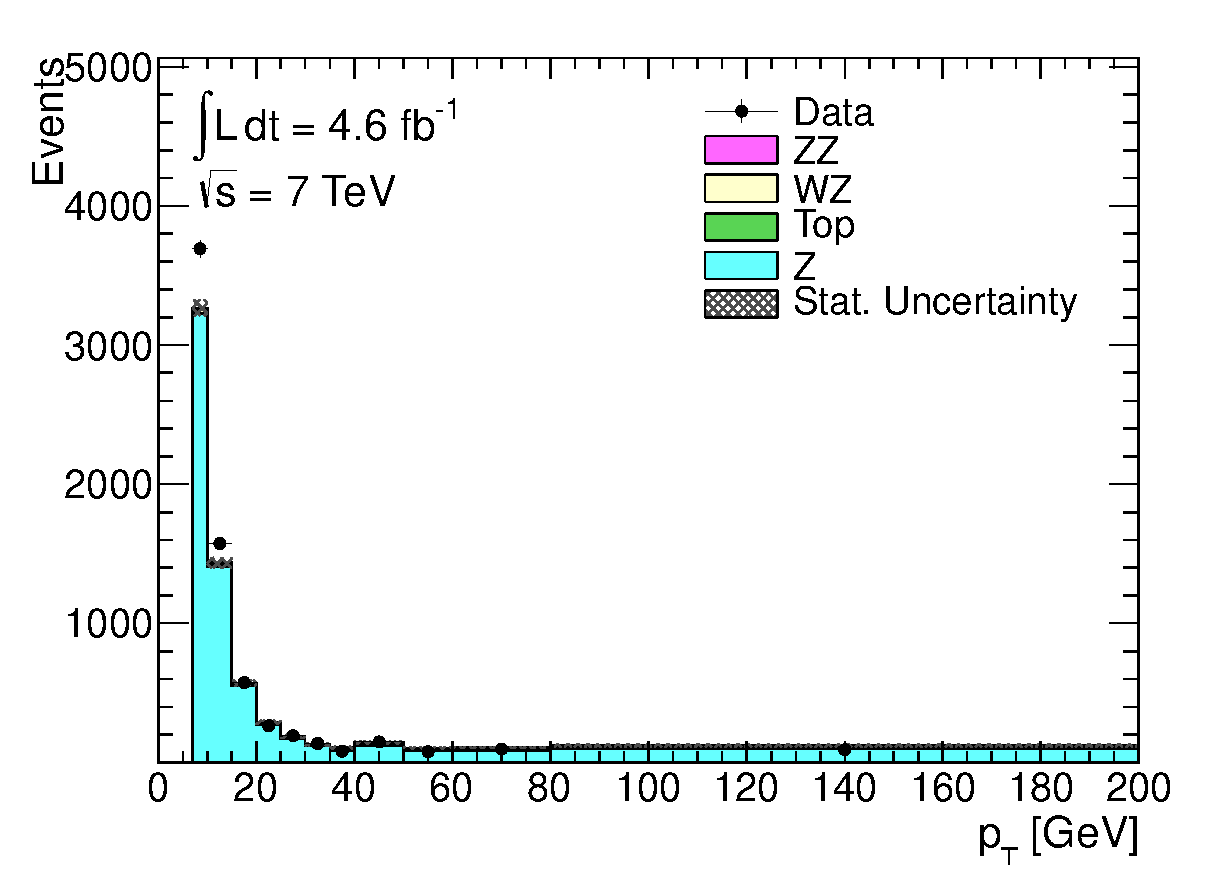
\includegraphics[width=0.47\textwidth]{ffDists7TeV/CentralEl_pt_L_lin}
        }
	\subfigure[Central Electron-Like-Jets]{
            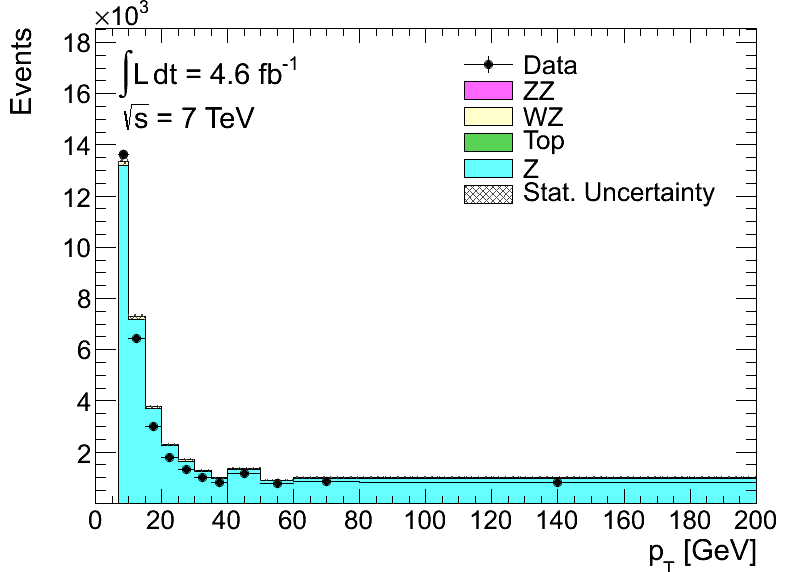
\includegraphics[width=0.47\textwidth]{ffDists7TeV/CentralEl_pt_J_lin}
        }
	\subfigure[Selected Forward Electrons]{
            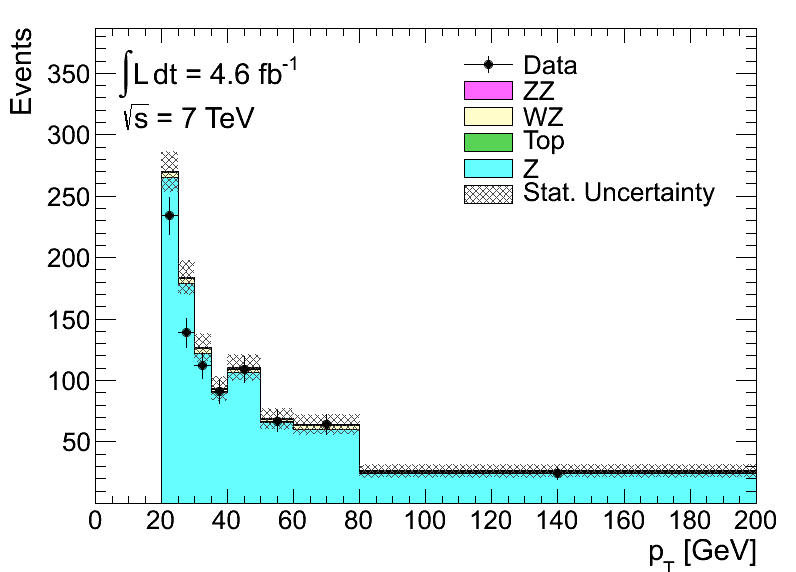
\includegraphics[width=0.47\textwidth]{ffDists7TeV/ForwardEl_pt_L_lin}
        }
	\subfigure[Forward Electron-Like-Jets]{
            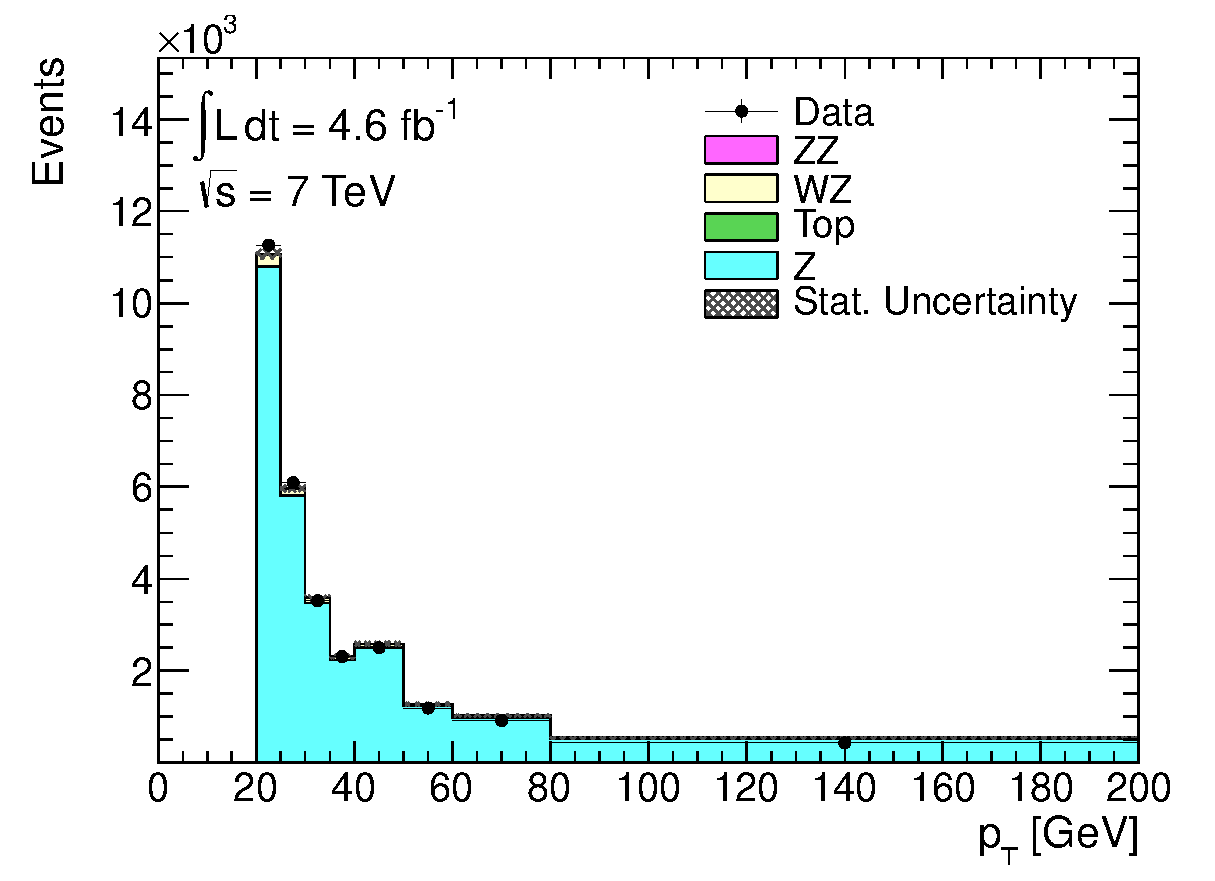
\includegraphics[width=0.47\textwidth]{ffDists7TeV/ForwardEl_pt_J_lin}
        }
	\subfigure[Selected Electrons]{
            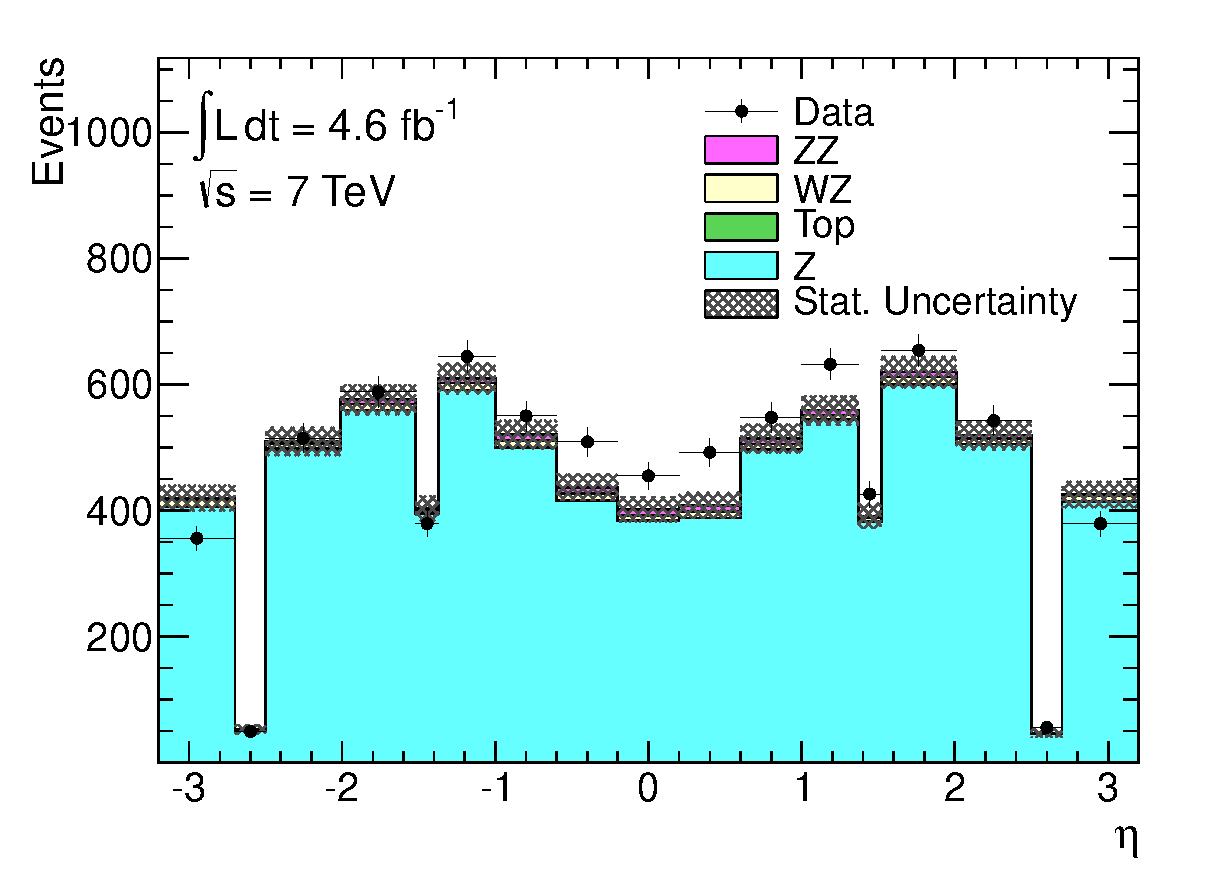
\includegraphics[width=0.47\textwidth]{ffDists7TeV/AllEl_eta_L_lin}
        }
	\subfigure[Electron-Like-Jets]{
            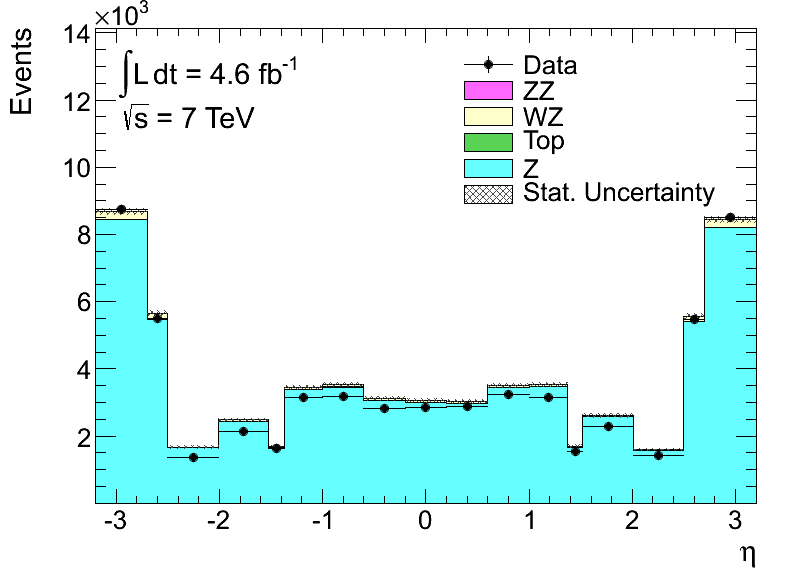
\includegraphics[width=0.47\textwidth]{ffDists7TeV/AllEl_eta_J_lin}
        }
    \caption[\pt\ and $\eta$ distributions for selected electrons $L$ and
    lepton-like-electrons $J$ in the \Z-tag sample for 7~\tev\ data.]
    {\pt\ and $\eta$ distributions for selected electrons $L$ and
    lepton-like-electrons $J$ in the \Z-tag sample for 7~\tev\ data. 
    For the \pt\ distributions, central and forward electrons are shown
    separately; for the $\eta$ distributions central and forward electrons are
    shown in the same plot.}
\label{fig:ljdist-el-seven} 
\end{figure}

\begin{figure}[h]
\centering
	\subfigure[Selected Central Electrons]{
            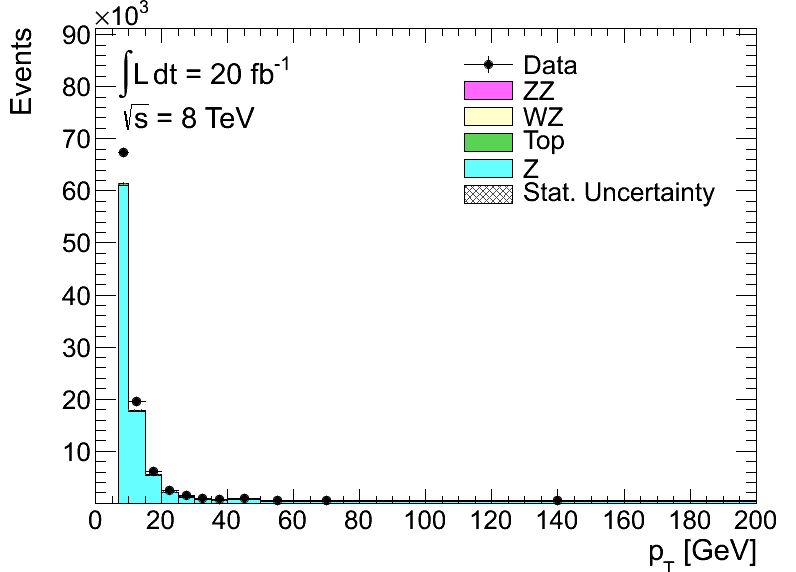
\includegraphics[width=0.47\textwidth]{ffDists8TeV/CentralEl_pt_L_lin}
        }
	\subfigure[Central Electron-Like-Jets]{
            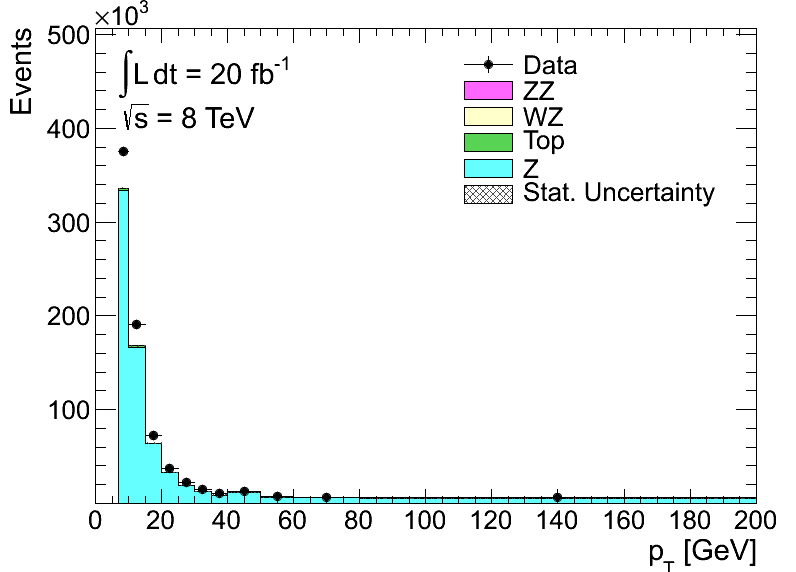
\includegraphics[width=0.47\textwidth]{ffDists8TeV/CentralEl_pt_J_lin}
        }
	\subfigure[Selected Central Electrons]{
            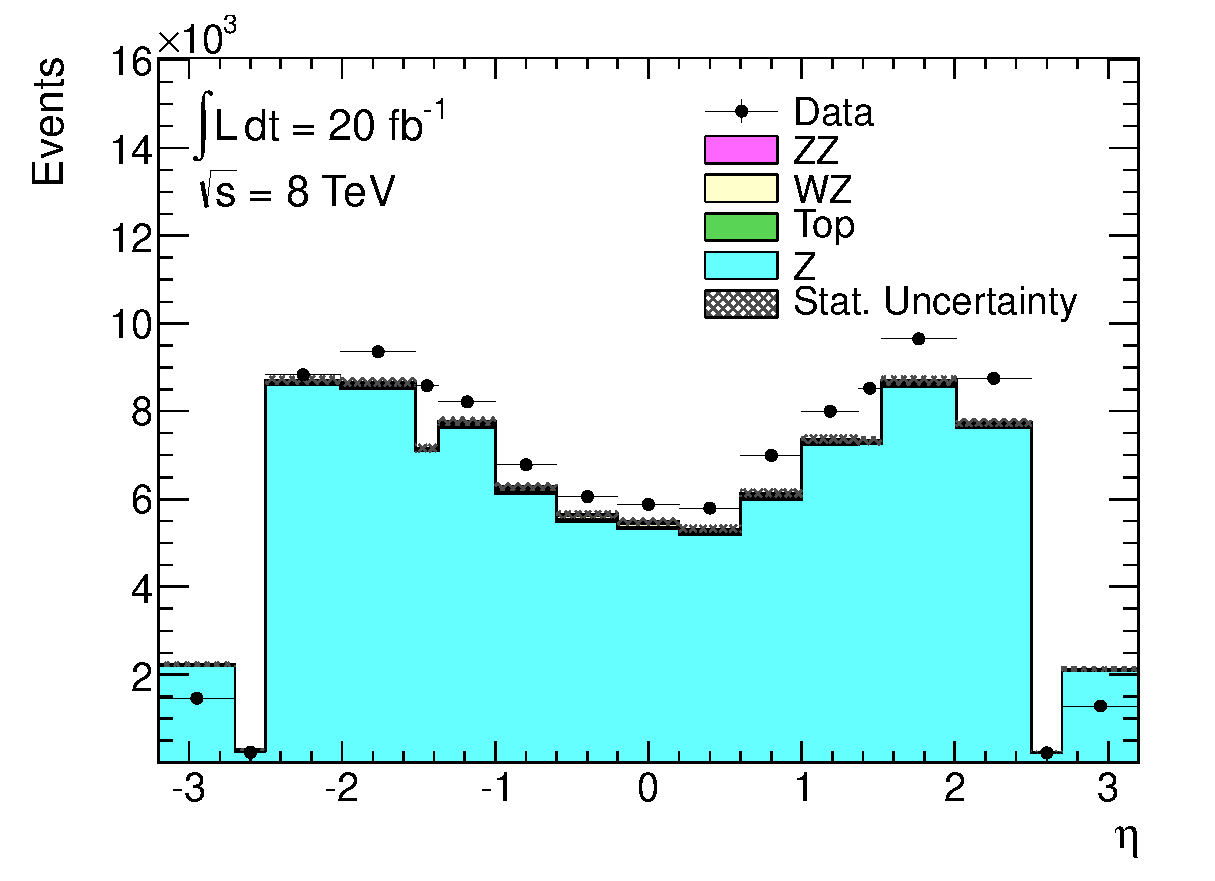
\includegraphics[width=0.47\textwidth]{ffDists8TeV/AllEl_eta_L_lin}
        }
	\subfigure[Central Electron-Like-Jets]{
            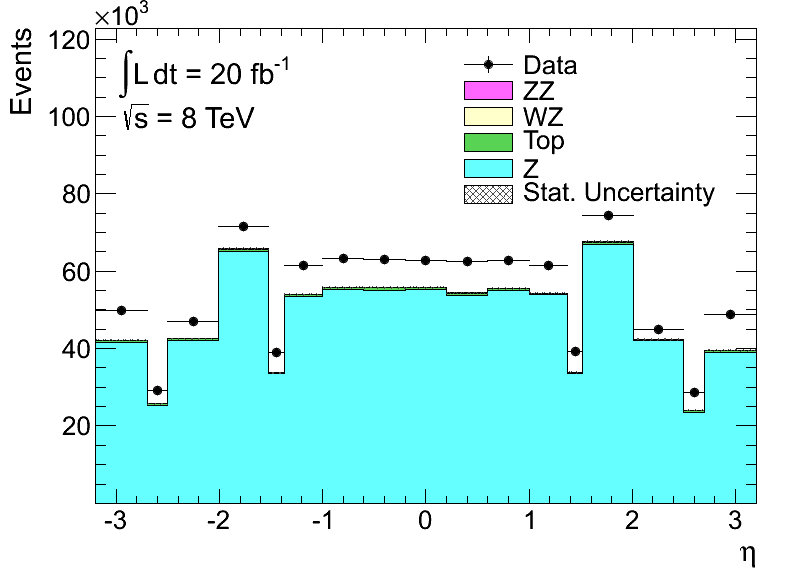
\includegraphics[width=0.47\textwidth]{ffDists8TeV/AllEl_eta_J_lin}
        }
    \caption[\pt\ and $\eta$ distributions for selected electrons $L$ and
    lepton-like-electrons $J$ in the \Z-tag sample for 8~\tev\ data.]
    {\pt\ and $\eta$ distributions for selected electrons $L$ and
    lepton-like-electrons $J$ in the \Z-tag sample for 8~\tev\ data. 
   }
\label{fig:ljdist-el-eight} 
\end{figure}

\begin{figure}[h]
\centering
\vspace{-8mm}
	\subfigure[Selected Central Muons]{
            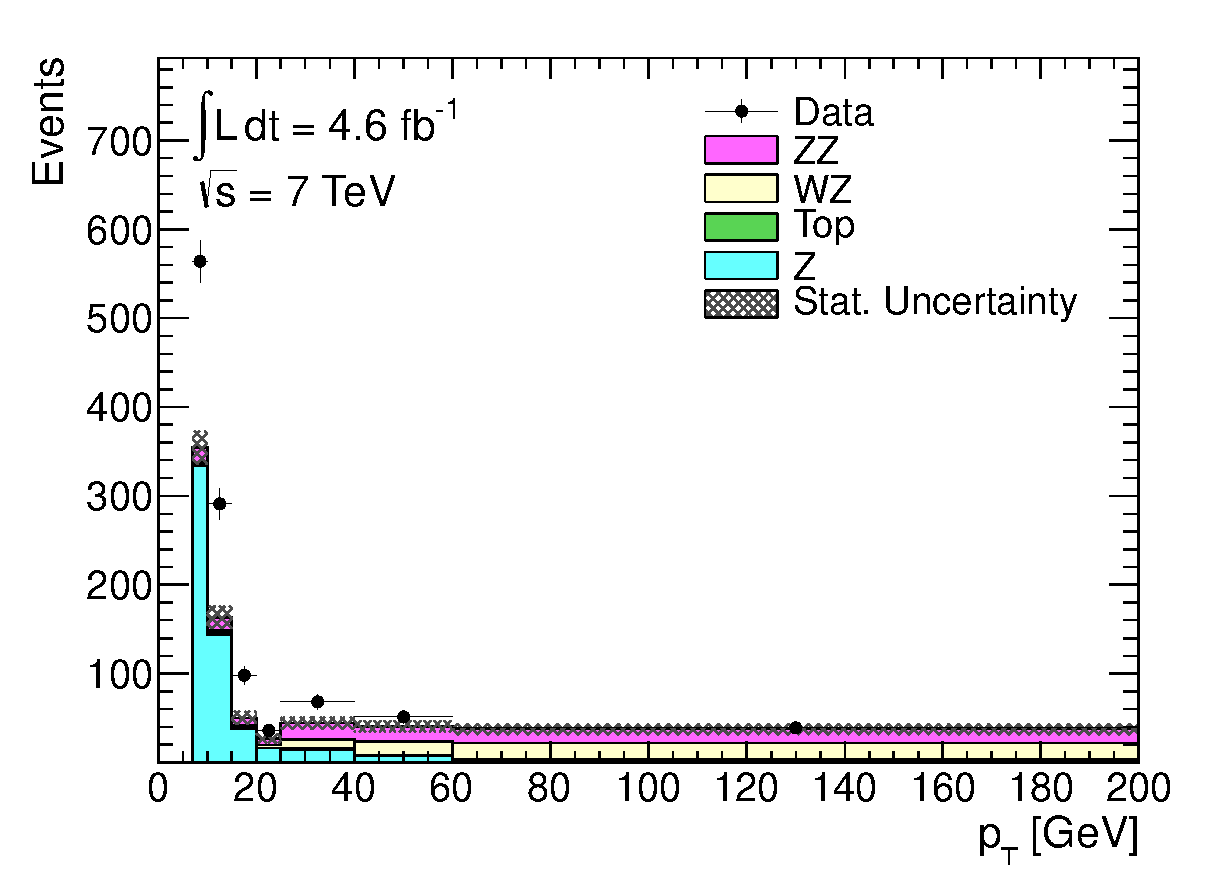
\includegraphics[width=0.47\textwidth]{ffDists7TeV/CentralMu_pt_L_lin}
        }
	\subfigure[Central Muon-Like-Jets]{
            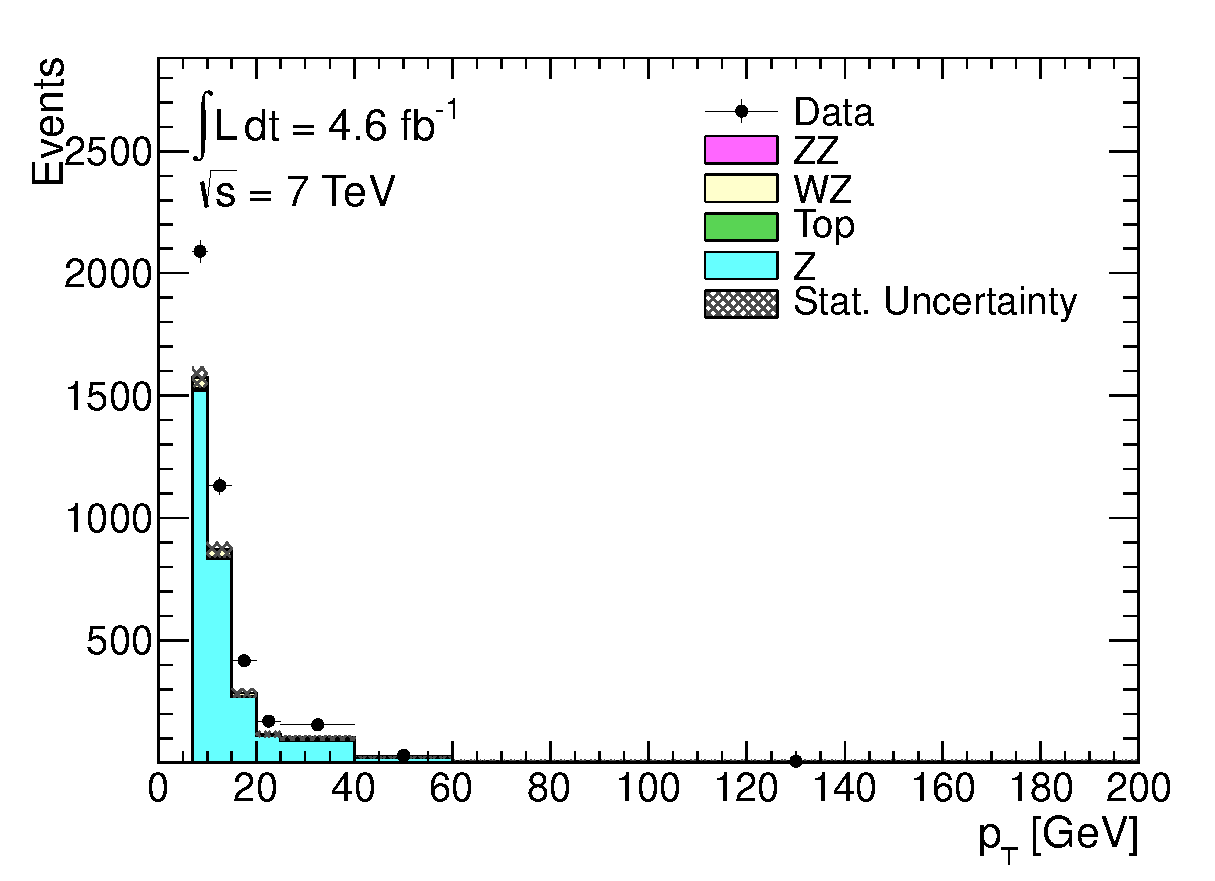
\includegraphics[width=0.47\textwidth]{ffDists7TeV/CentralMu_pt_J_lin}
        }
	\subfigure[Selected Forward Muons]{
            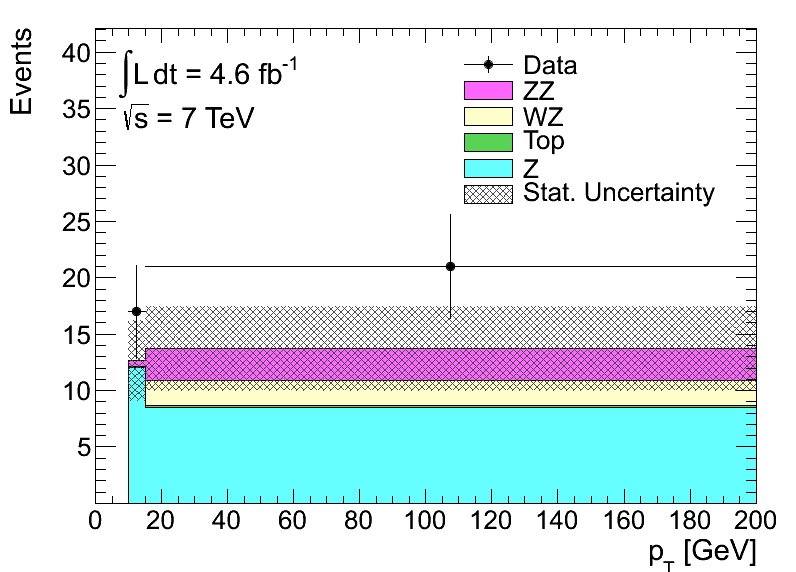
\includegraphics[width=0.47\textwidth]{ffDists7TeV/ForwardMu_pt_L_lin}
        }
	\subfigure[Forward Muon-Like-Jets]{
            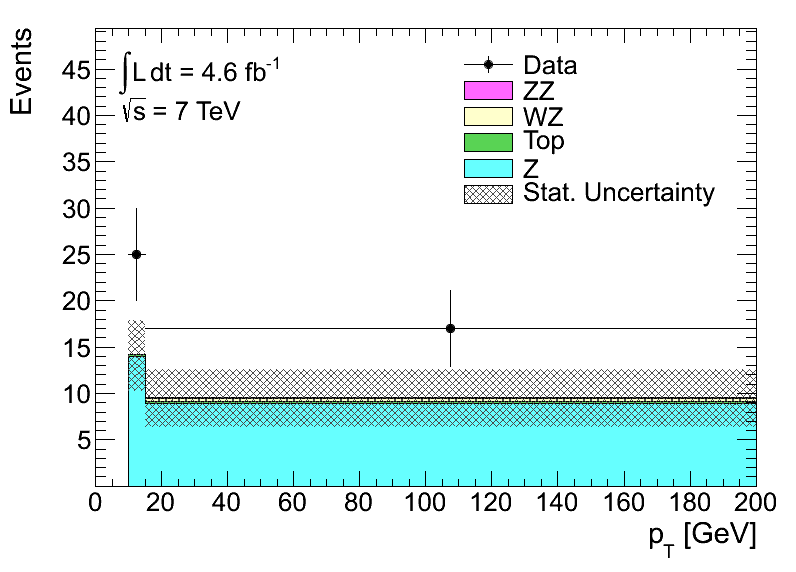
\includegraphics[width=0.47\textwidth]{ffDists7TeV/ForwardMu_pt_J_lin}
        }
	\subfigure[Selected Calorimeter-Tagged Muons]{
            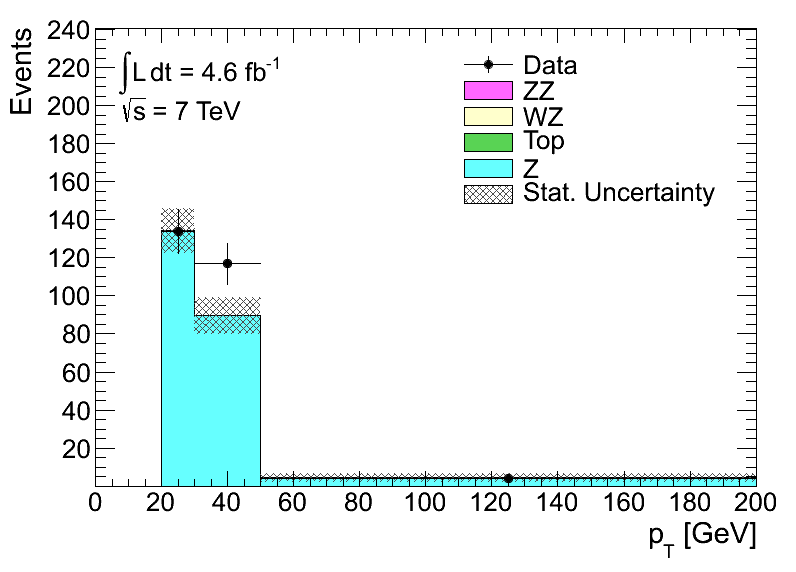
\includegraphics[width=0.47\textwidth]{ffDists7TeV/CaloMu_pt_J_lin}
        }
	\subfigure[Calorimeter-Tagged Muon-Like-Jets]{
            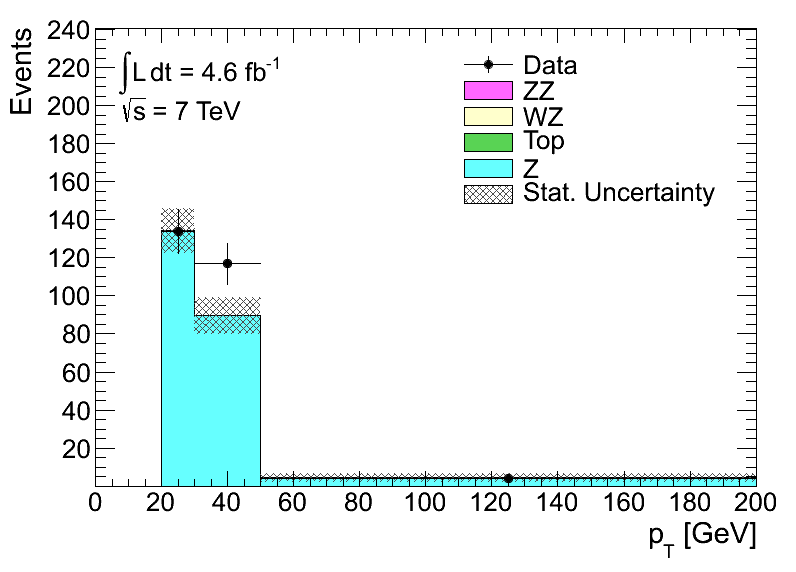
\includegraphics[width=0.47\textwidth]{ffDists7TeV/CaloMu_pt_J_lin}
        }
	\subfigure[Selected Muons]{
            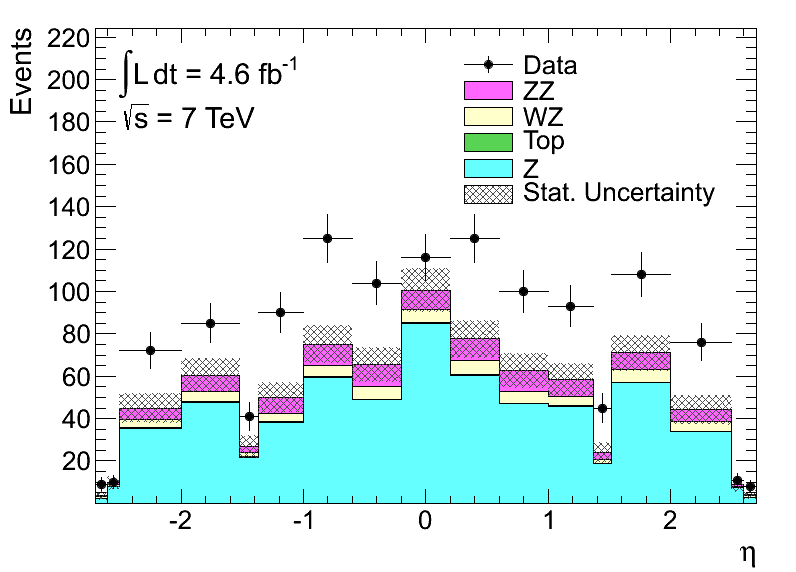
\includegraphics[width=0.47\textwidth]{ffDists7TeV/AllMu_eta_L_lin}
        }
	\subfigure[Muon-Like-Jets]{
            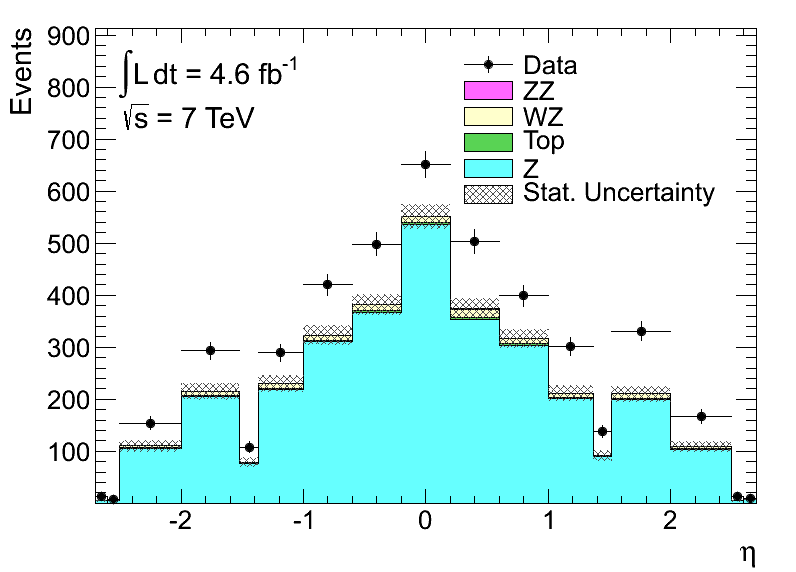
\includegraphics[width=0.47\textwidth]{ffDists7TeV/AllMu_eta_J_lin}
        }
    \caption[\pt\ and $\eta$ distributions for selected muons $L$ and
    lepton-like-muons $J$ in the \Z-tag sample for 7~\tev\ data.]
    {\small \pt\ and $\eta$ distributions for selected muons $L$ and
    lepton-like-muons $J$ in the \Z-tag sample for 7~\tev\ data. 
    For the \pt\ distributions, central, forward and calorimeter-tagged muons are shown
    separately; for the $\eta$ distributions all muons are
    shown in the same plot.}
\label{fig:ljdist-mu-seven} 
\end{figure}

\begin{figure}[h]
\centering
\vspace{-8mm}
	\subfigure[Selected Central Muons]{
            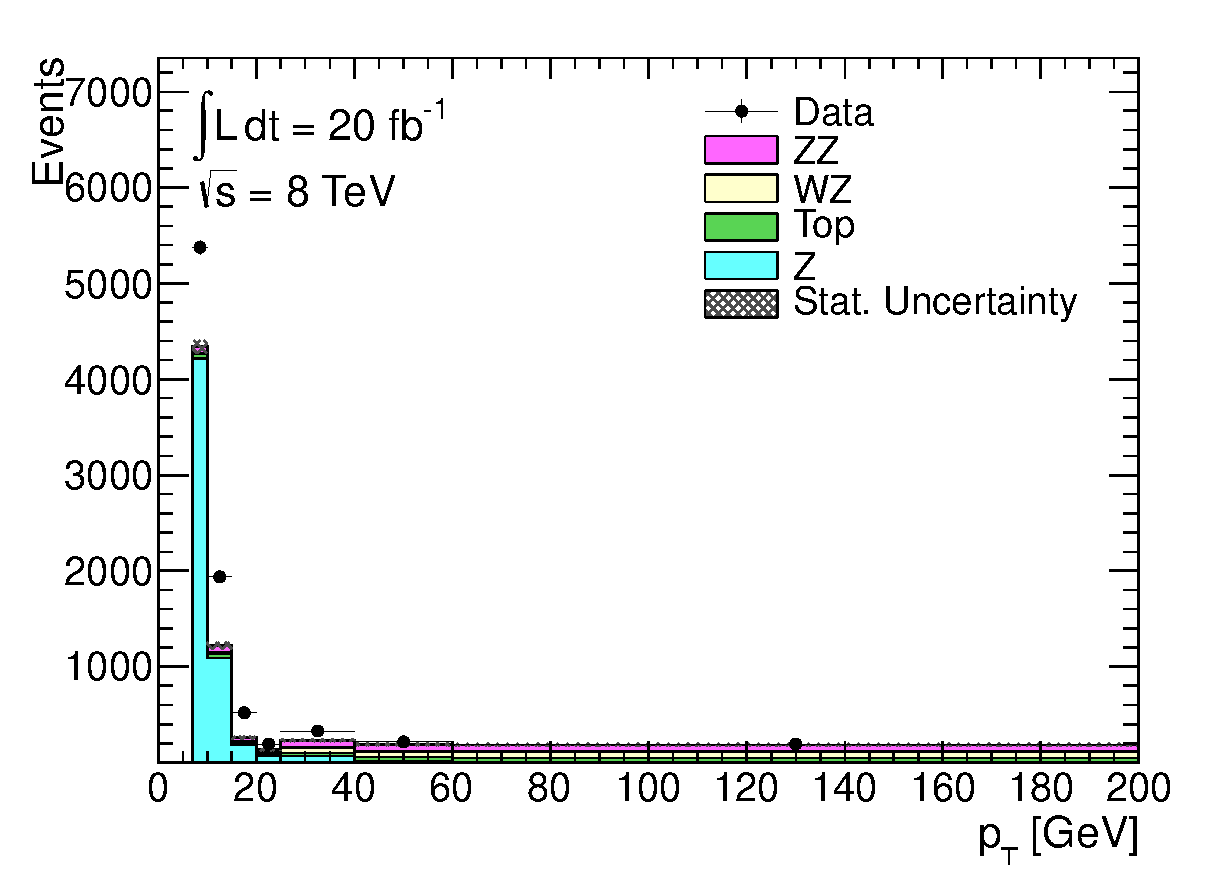
\includegraphics[width=0.47\textwidth]{ffDists8TeV/CentralMu_pt_L_lin}
        }
	\subfigure[Central Muon-Like-Jets]{
            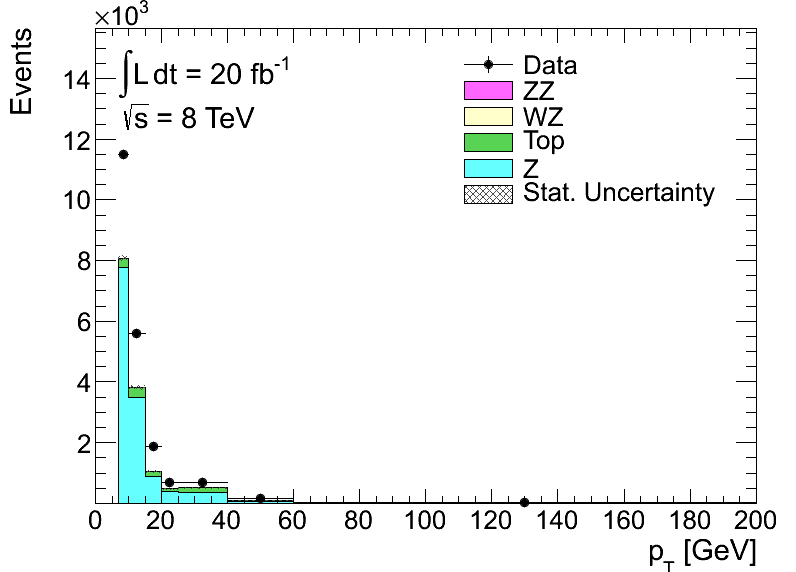
\includegraphics[width=0.47\textwidth]{ffDists8TeV/CentralMu_pt_J_lin}
        }
	\subfigure[Selected Forward Muons]{
            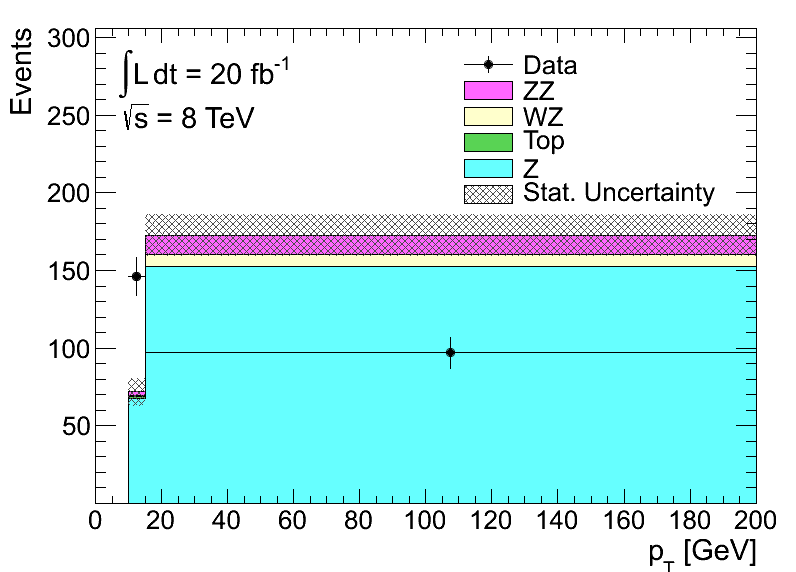
\includegraphics[width=0.47\textwidth]{ffDists8TeV/ForwardMu_pt_L_lin}
        }
	\subfigure[Forward Muon-Like-Jets]{
            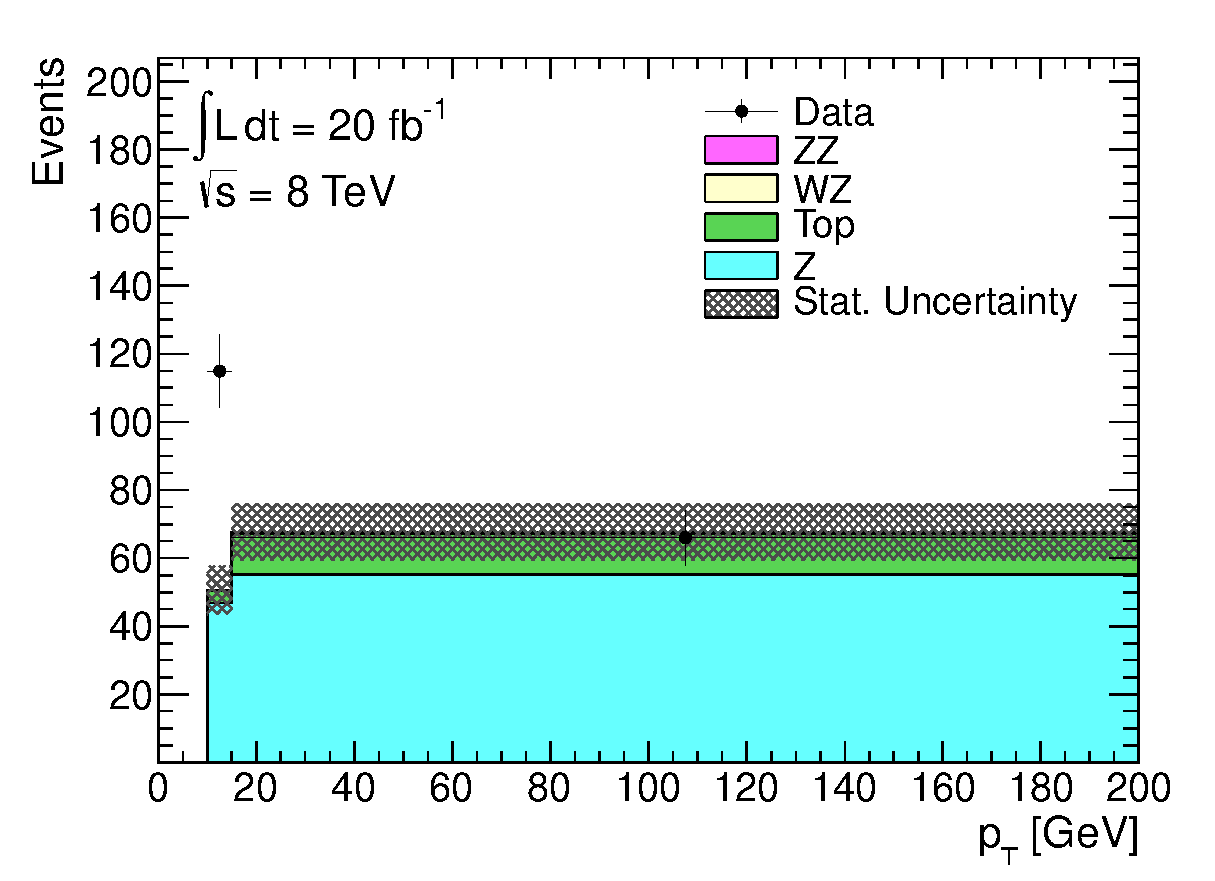
\includegraphics[width=0.47\textwidth]{ffDists8TeV/ForwardMu_pt_J_lin}
        }
	\subfigure[Selected Calorimeter-Tagged Muons]{
            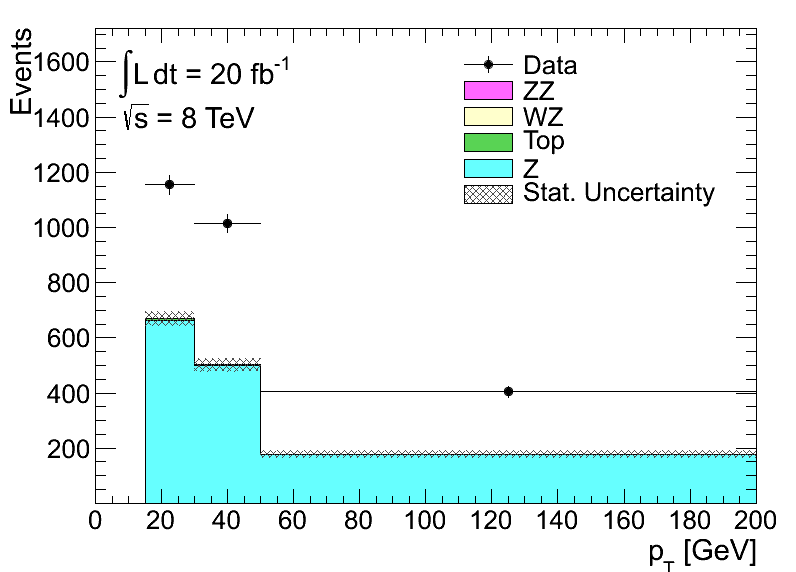
\includegraphics[width=0.47\textwidth]{ffDists8TeV/CaloMu_pt_J_lin}
        }
	\subfigure[Calorimeter-Tagged Muon-Like-Jets]{
            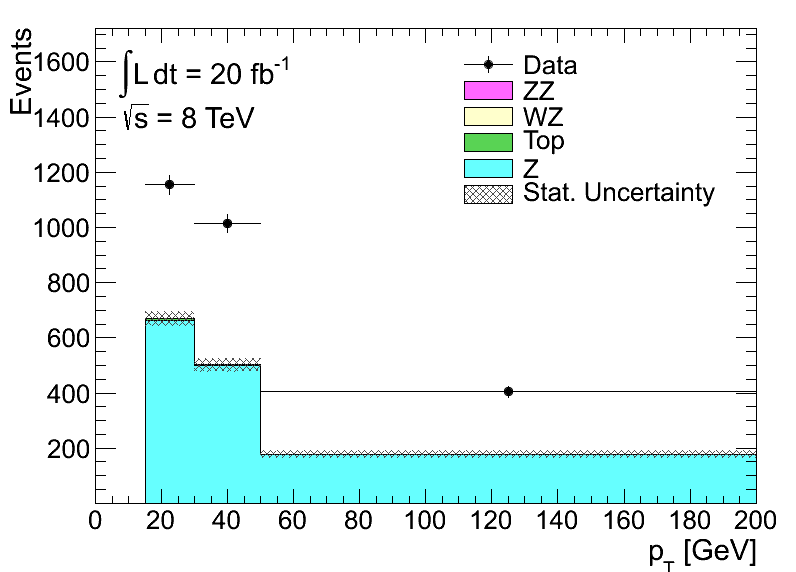
\includegraphics[width=0.47\textwidth]{ffDists8TeV/CaloMu_pt_J_lin}
        }
	\subfigure[Selected Muons]{
            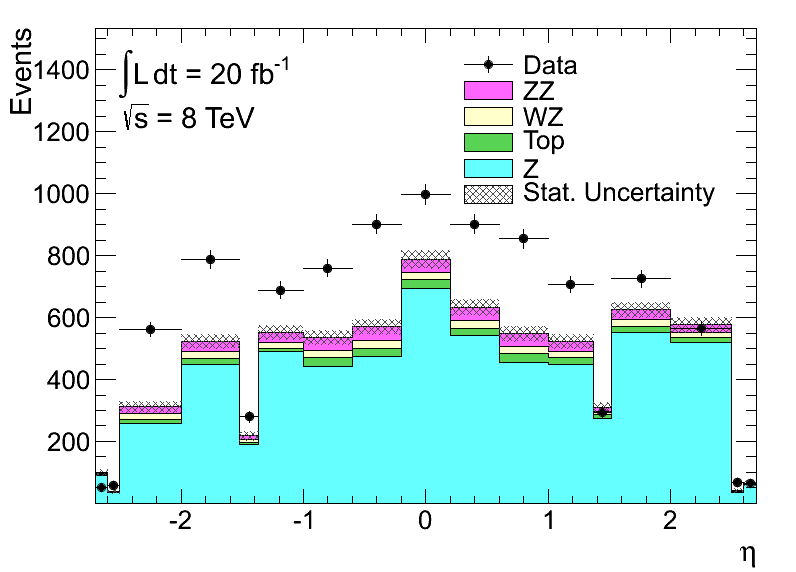
\includegraphics[width=0.47\textwidth]{ffDists8TeV/AllMu_eta_L_lin}
        }
	\subfigure[Muon-Like-Jets]{
            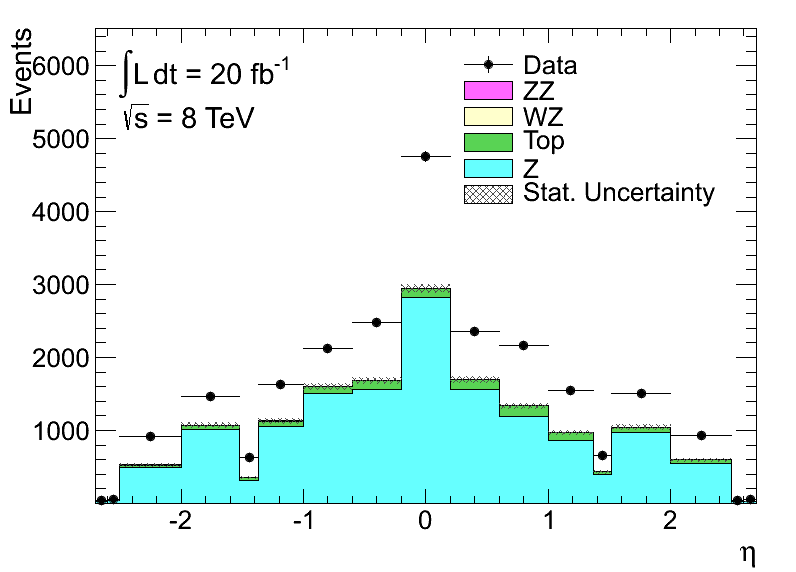
\includegraphics[width=0.47\textwidth]{ffDists8TeV/AllMu_eta_J_lin}
        }
    \caption[\pt\ and $\eta$ distributions for selected muons $L$ and
    lepton-like-muons $J$ in the \Z-tag sample for 8~\tev\ data.]
    {\small \pt\ and $\eta$ distributions for selected muons $L$ and
    lepton-like-muons $J$ in the \Z-tag sample for 8~\tev\ data. 
    For the \pt\ distributions, central, forward and calorimeter-tagged muons are shown
    separately; for the $\eta$ distributions all muons are
    shown in the same plot.}
\label{fig:ljdist-mu-eight} 
\end{figure}


The observed \fakefactor s for electrons are shown in~\fig{ff-el-seven} for the
7~\tev\ analysis and in~\fig{ff-el-eight} for the 8~\tev\ analysis; the \fakefactor s
for muons are shown in~\fig{ff-mu-seven} for the
7~\tev\ analysis and in~\fig{ff-mu-eight} for the 8~\tev\ analysis. The
\ffactor\ estimated from \mc\ (blue triangles) is in reasonable agreement with
the \ffactor\ measured in data (black points). For the calculation of the
background, no use is made of the \ffactor\ estimated from \mc. The average \FF
s, used as the numerator in~\eqn{factorised-ff}, are given in~\tab{average-ff}.

\begin{table}[htbp]
  \centering
  \small
  \begin{tabular}{lcc} 
    \hline\hline
    Lepton & $<\FF>$ 7~\tev &  $<\FF>$ 8~\tev \\
    \hline
    Central Electron            & \measStat{0.215}{\errSym{0.003}} & \measStat{0.133}{\errSym{0.001}}\\
    Forward Electron            & \measStat{0.030}{\errSym{0.001}} & - \\
    Central Muon                & \measStat{0.250}{\errSym{0.010}} & \measStat{0.395}{\errSym{0.005}}\\
    Forward Muon                & \measStat{0.782}{\errSym{0.199}} & \measStat{1.212}{\errSym{0.128}}\\
    Calorimeter-Tagged Muon     & \measStat{0.123}{\errSym{0.024}} & \measStat{0.098}{\errSym{0.007}} \\
    \hline\hline
  \end{tabular}
  \caption{Average \ffactor s for different lepton types.}
  \label{table:average-ff}
\end{table}

\begin{figure}[h]
\centering
	\subfigure[Central Electrons]{
            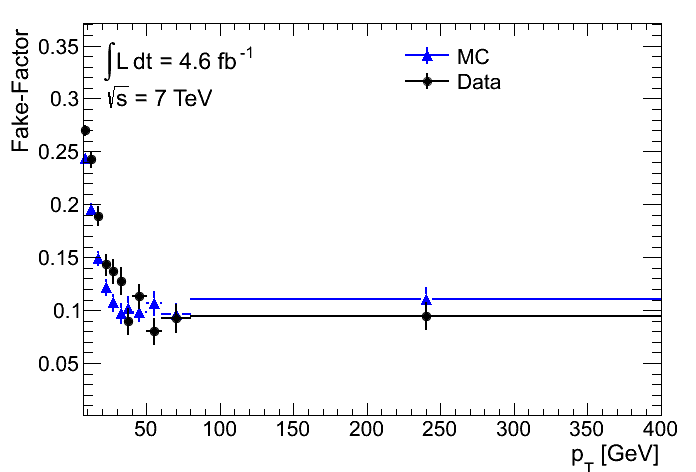
\includegraphics[width=0.47\textwidth]{FakeFactors7TeV/FF_CentralEl_pt_J_lin}
        }
	\subfigure[Forward Electrons]{
            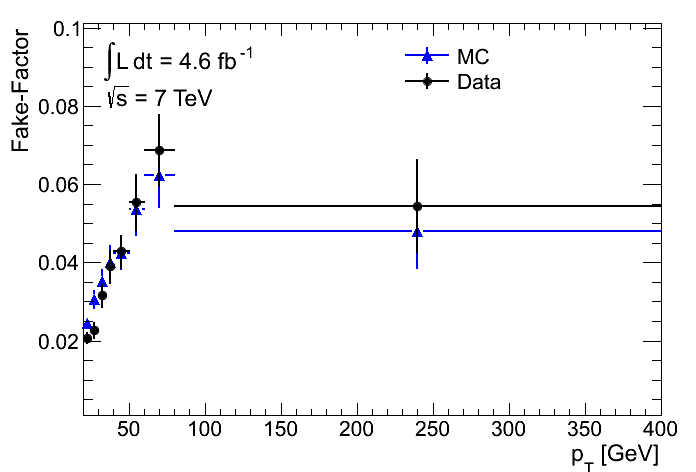
\includegraphics[width=0.47\textwidth]{FakeFactors7TeV/FF_ForwardEl_pt_J_lin}
        }
	\subfigure[All Electrons]{
            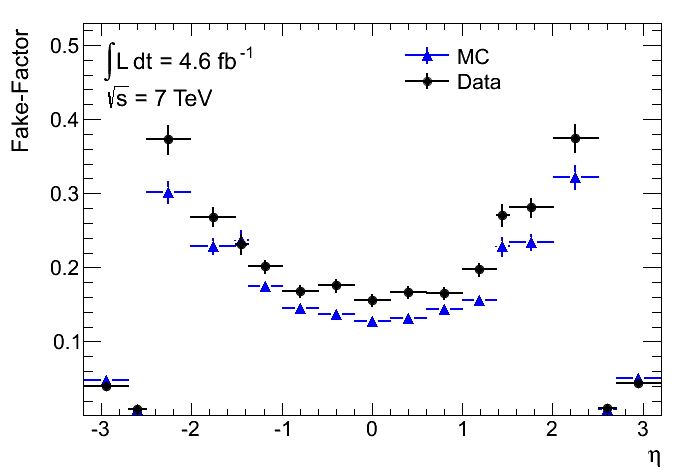
\includegraphics[width=0.47\textwidth]{FakeFactors7TeV/FF_AllEl_eta_J_lin}
        }
    \caption[Electron \FakeFactor s as a function of \pt\ and $\eta$ for 7~\tev\ data.]
    {Electron \FakeFactor s as a function of \pt\ and $\eta$ for 7~\tev\ data. 
    For the distributions as a function of \pt\, central and forward electrons are shown
    separately; for the $\eta$ distributions the \ffactor\ for central and forward electrons are
    shown in the same plot. The black points show the \ffactor\ measured in
    data; the blue triangles show the value estimated by \mc.}
\label{fig:ff-el-seven} 
\end{figure}

\begin{figure}[h]
\centering
\vspace{-8mm}
	\subfigure[Central Muons]{
            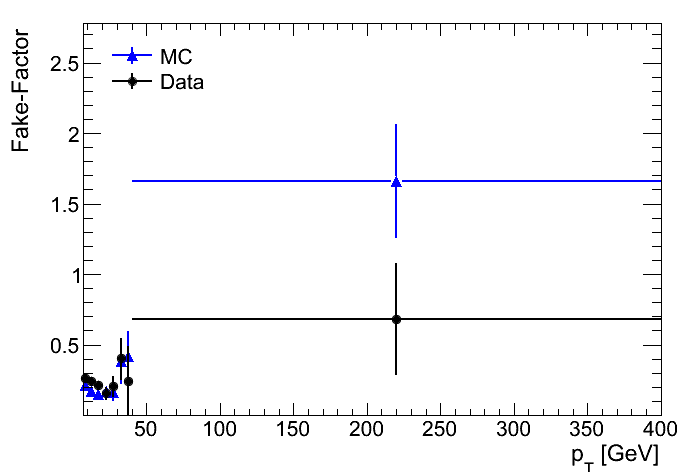
\includegraphics[width=0.47\textwidth]{FakeFactors7TeV/FF_CentralMu_pt_J_lin}
        }
	\subfigure[Forward Muons]{
            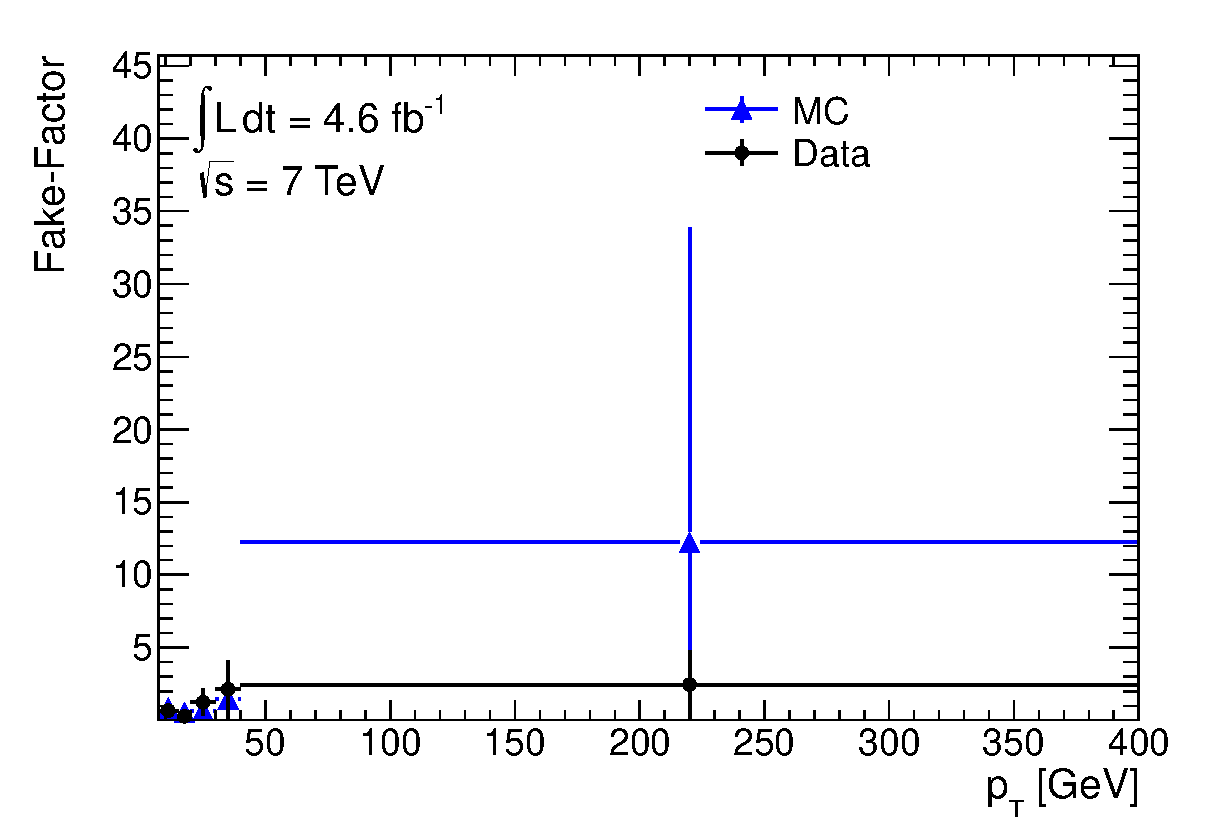
\includegraphics[width=0.47\textwidth]{FakeFactors7TeV/FF_ForwardMu_pt_J_lin}
        }
	\subfigure[Calorimeter-Tagged Muons]{
            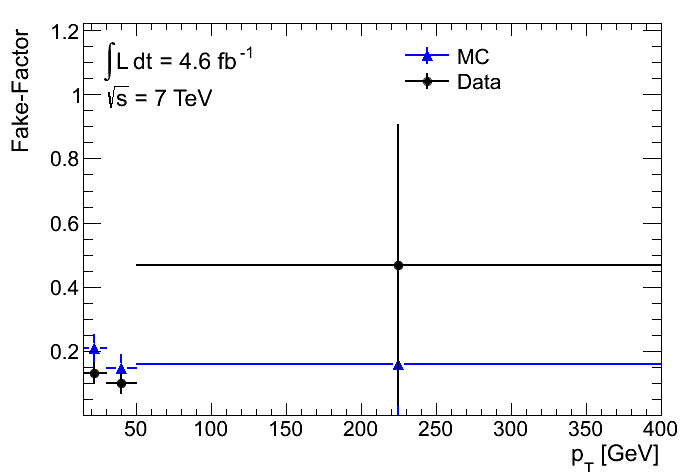
\includegraphics[width=0.47\textwidth]{FakeFactors7TeV/FF_CaloMu_pt_J_lin}
        }
	\subfigure[All Muons]{
            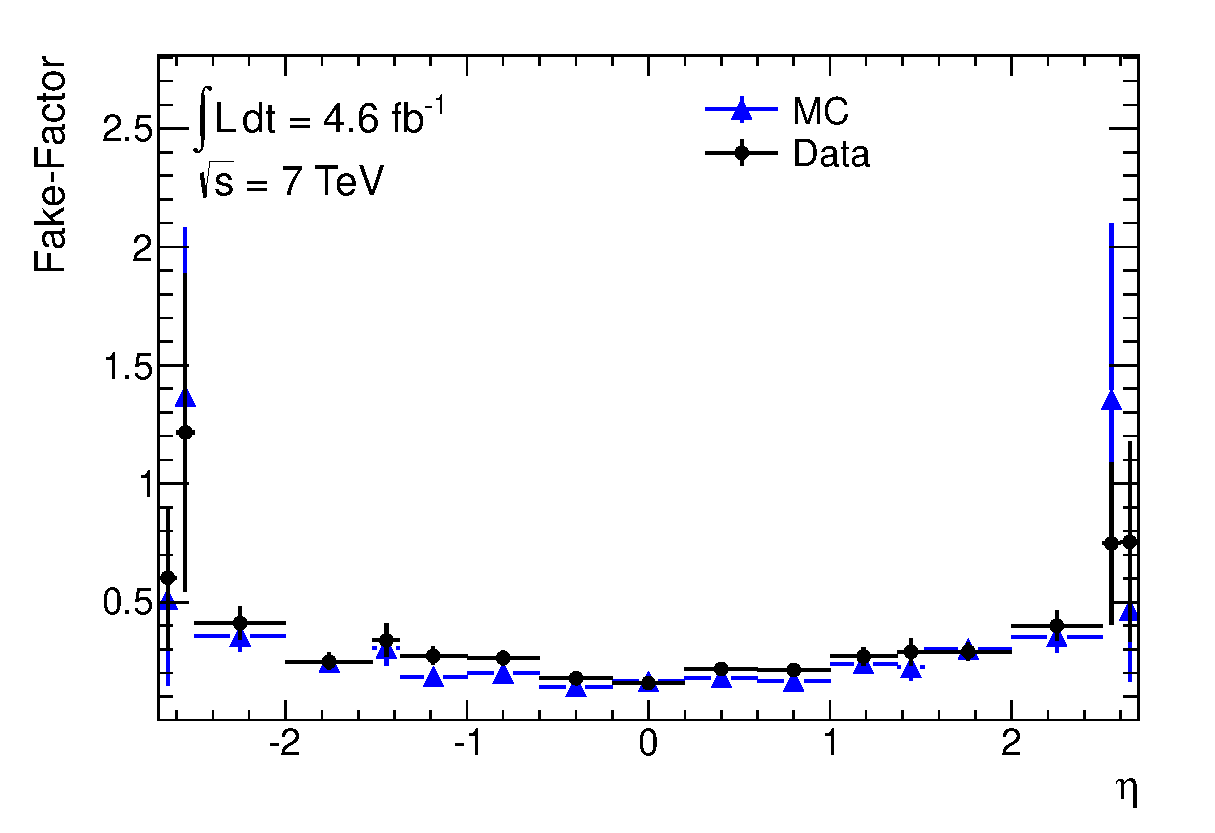
\includegraphics[width=0.47\textwidth]{FakeFactors7TeV/FF_AllMu_eta_J_lin}
        }
    \caption[Muon \FakeFactor s as a function of \pt\ and $\eta$ for 7~\tev\ data.]
    {Muon \FakeFactor s as a function of \pt\ and $\eta$ for 7~\tev\ data. 
    For the distributions as a function of \pt\, central, forward and calorimeter-tagged muons are shown
    separately; for the $\eta$ distributions the \ffactor\ all muons are
    shown in the same plot.The black points show the \ffactor\ measured in
    data; the blue triangles show the value estimated by \mc.}
\label{fig:ff-mu-seven} 
\end{figure}

\begin{figure}[h]
\centering
	\subfigure[Central Electrons]{
            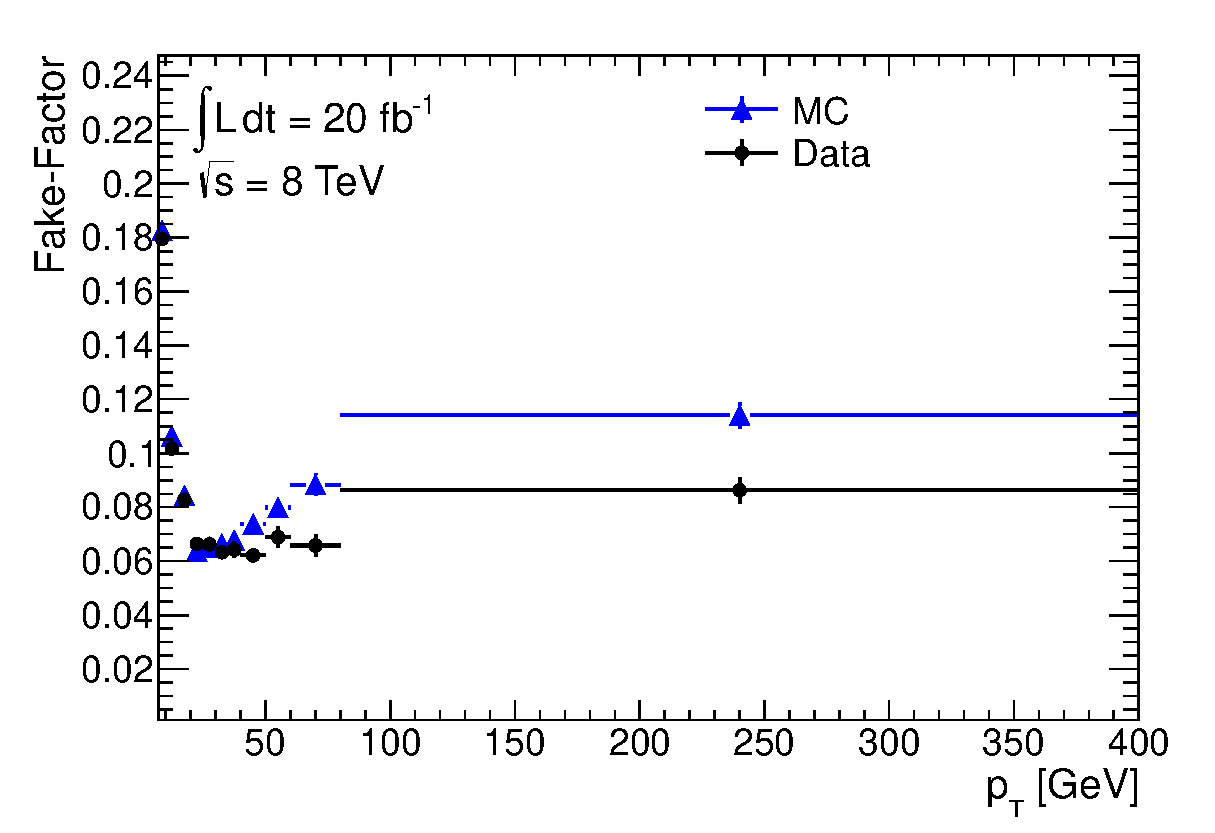
\includegraphics[width=0.47\textwidth]{FakeFactors8TeV/FF_CentralEl_pt_J_lin}
        }
	%\subfigure[Forward Electrons]{
            %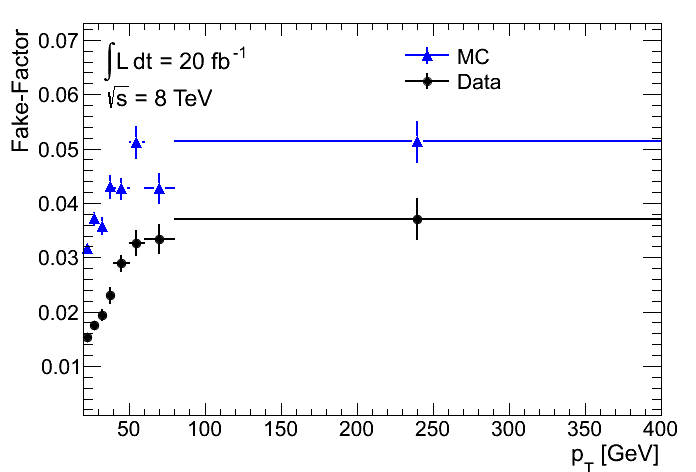
\includegraphics[width=0.47\textwidth]{FakeFactors8TeV/FF_ForwardEl_pt_J_lin}
        %}
	\subfigure[Central Electrons]{
            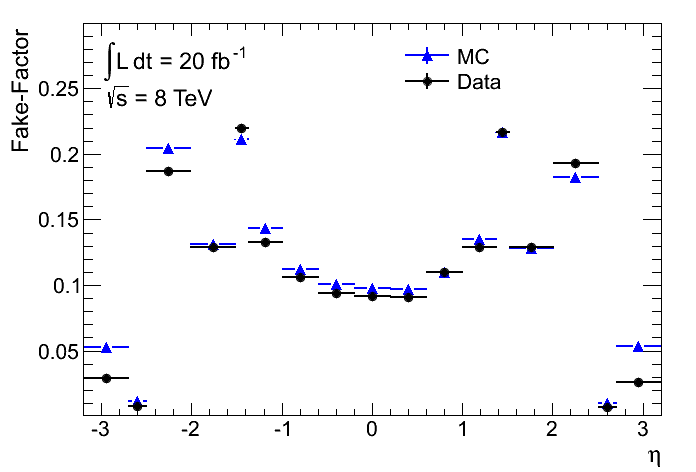
\includegraphics[width=0.47\textwidth]{FakeFactors8TeV/FF_AllEl_eta_J_lin}
        }
    \caption[Electron \FakeFactor s as a function of \pt\ and $\eta$ for 8~\tev\ data.]
    {Electron \FakeFactor s as a function of \pt\ and $\eta$ for 8~\tev\ data. 
    The black points show the \ffactor\ measured in
    data; the blue triangles show the value estimated by \mc.}
\label{fig:ff-el-eight} 
\end{figure}

\begin{figure}[h]
\centering
\vspace{-8mm}
	\subfigure[Central Muons]{
            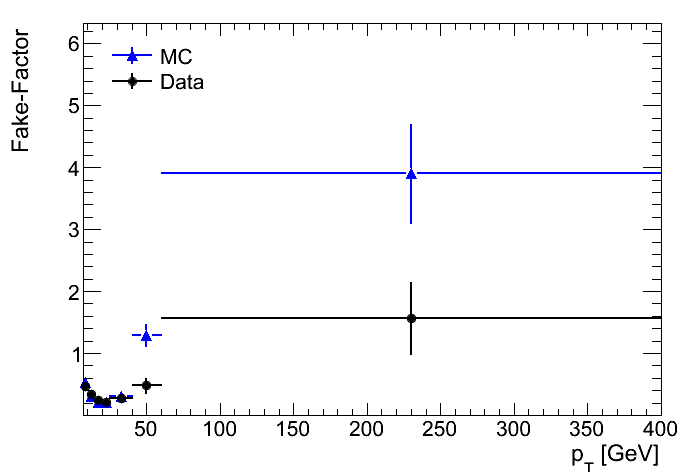
\includegraphics[width=0.47\textwidth]{FakeFactors8TeV/FF_CentralMu_pt_J_lin}
        }
	\subfigure[Forward Muons]{
            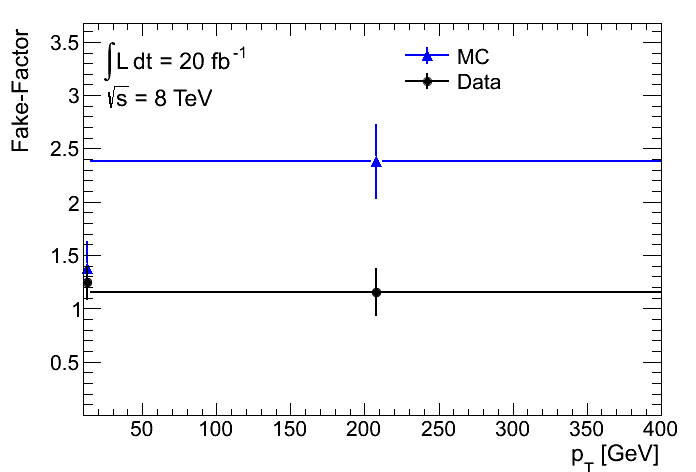
\includegraphics[width=0.47\textwidth]{FakeFactors8TeV/FF_ForwardMu_pt_J_lin}
        }
	\subfigure[Calorimeter-Tagged Muons]{
            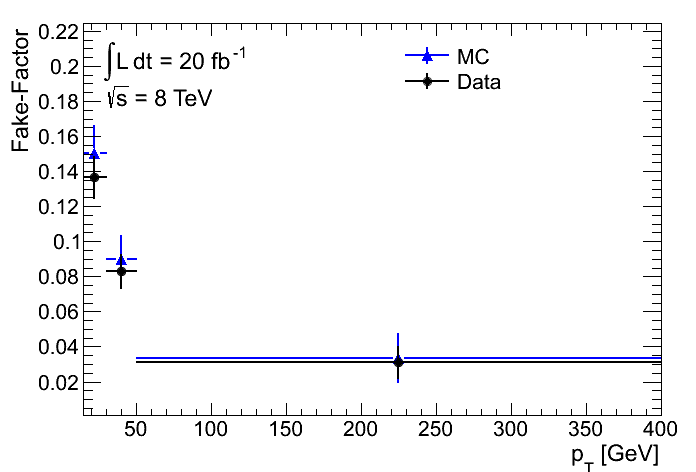
\includegraphics[width=0.47\textwidth]{FakeFactors8TeV/FF_CaloMu_pt_J_lin}
        }
	\subfigure[All Muons]{
            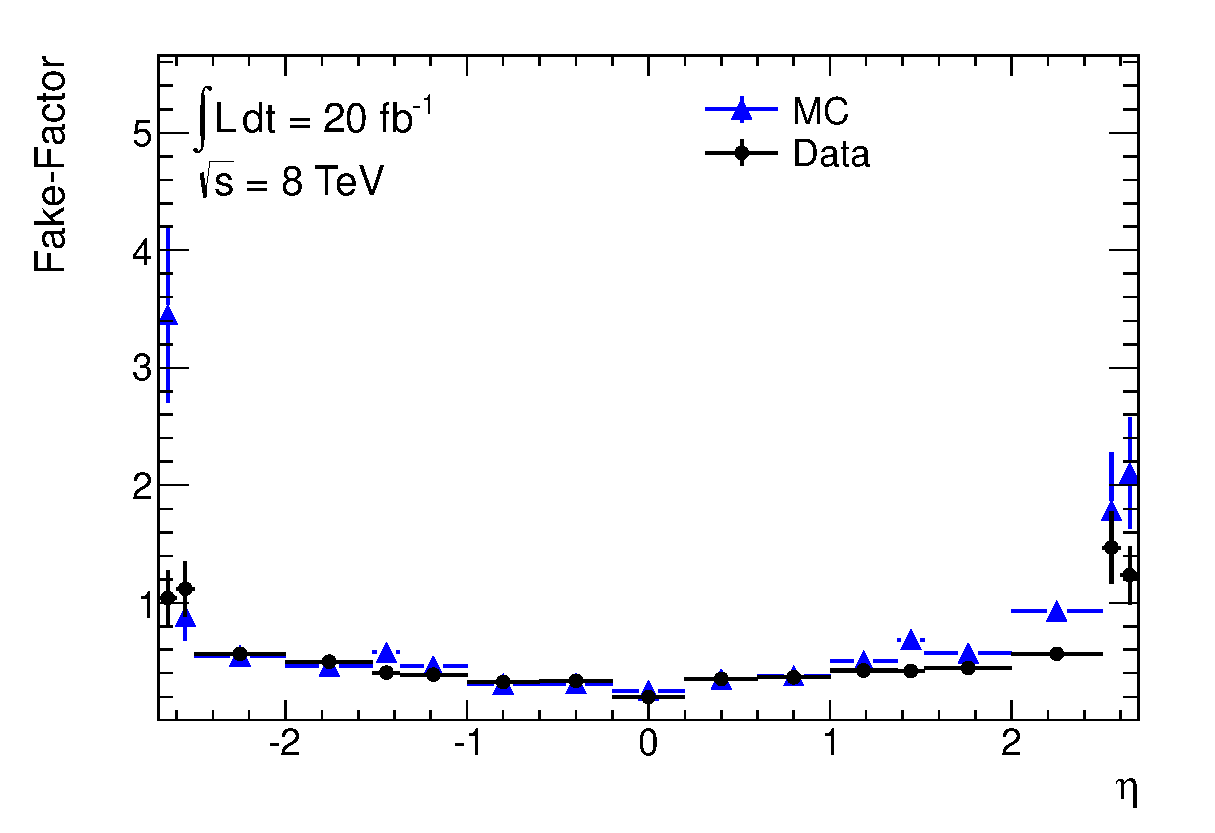
\includegraphics[width=0.47\textwidth]{FakeFactors8TeV/FF_AllMu_eta_J_lin}
        }
    \caption[Muon \FakeFactor s as a function of \pt\ and $\eta$ for 8~\tev\ data.]
    {Muon \FakeFactor s as a function of \pt\ and $\eta$ for 8~\tev\ data. 
    For the distributions as a function of \pt\, central, forward and calorimeter-tagged muons are shown
    separately; for the $\eta$ distributions the \ffactor\ all muons are
    shown in the same plot.The black points show the \ffactor\ measured in
    data; the blue triangles show the value estimated by \mc.}
\label{fig:ff-mu-eight} 
\end{figure}

%\begin{figure}[h]
%\centering
%	\subfigure[Central Electrons]{
%            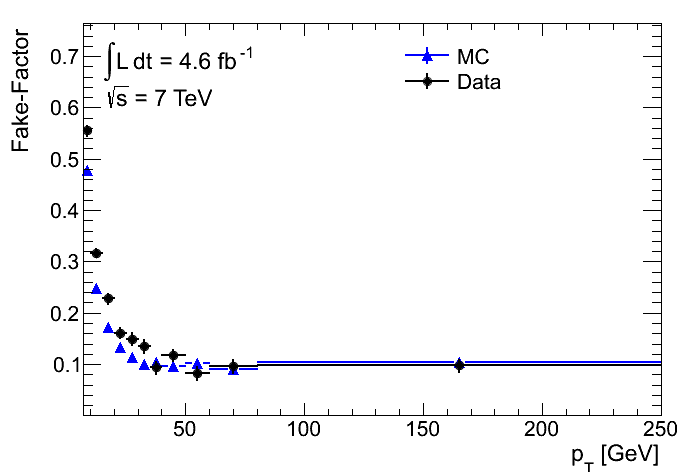
\includegraphics[width=0.47\textwidth]{FakeFactors/FF_CentralEl_pt_B_lin}
%        }
%	\subfigure[Forward Electrons]{
%            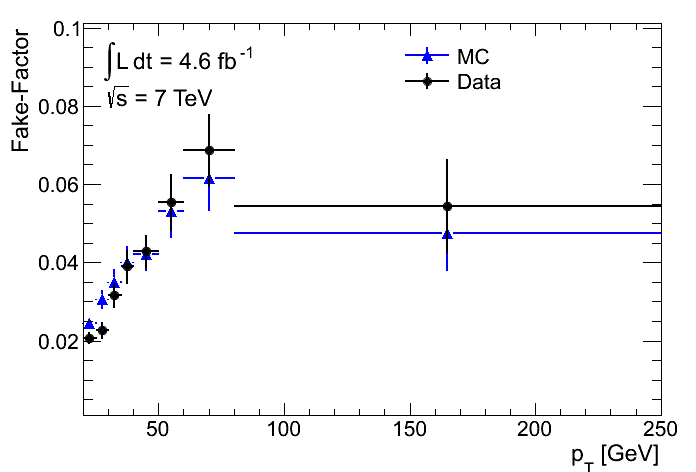
\includegraphics[width=0.47\textwidth]{FakeFactors/FF_ForwardEl_pt_B_lin}
%        }
%	\subfigure[All Electrons]{
%            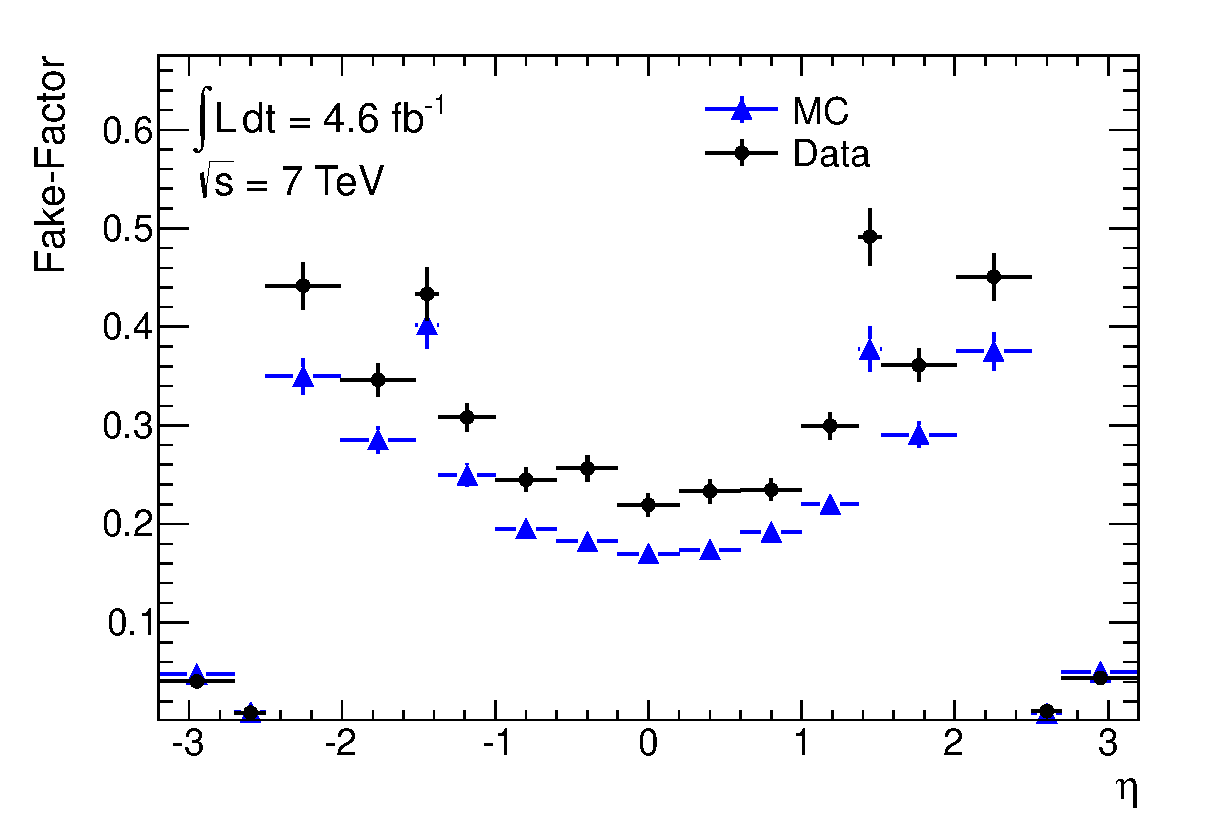
\includegraphics[width=0.47\textwidth]{FakeFactors/FF_AllEl_eta_B_lin}
%        }
%    \caption[Electron \FakeFactor s as a function of \pt\ and $\eta$ for 7~\tev\ data.]
%    {Electron \FakeFactor s as a function of \pt\ and $\eta$ for 7~\tev\ data. 
%    For the distributions as a function of \pt\, central and forward electrons are shown
%    separately; for the $\eta$ distributions the \ffactor\ for central and forward electrons are
%    shown in the same plot. The black points show the \ffactor\ measured in
%    data; the blue triangles show the value estimated by \mc.}
%\label{fig:ff-el-seven} 
%\end{figure}

%\begin{figure}[h]
%\centering
%\vspace{-8mm}
%	\subfigure[Central Muons]{
%            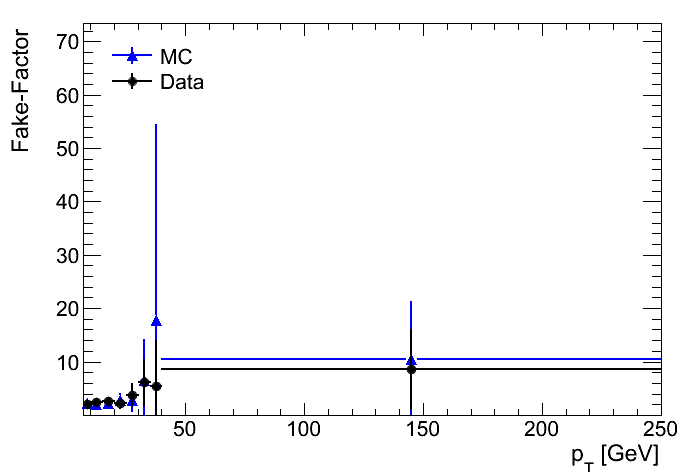
\includegraphics[width=0.47\textwidth]{FakeFactors/FF_CentralMu_pt_B_lin}
%        }
%	\subfigure[Forward Muons]{
%            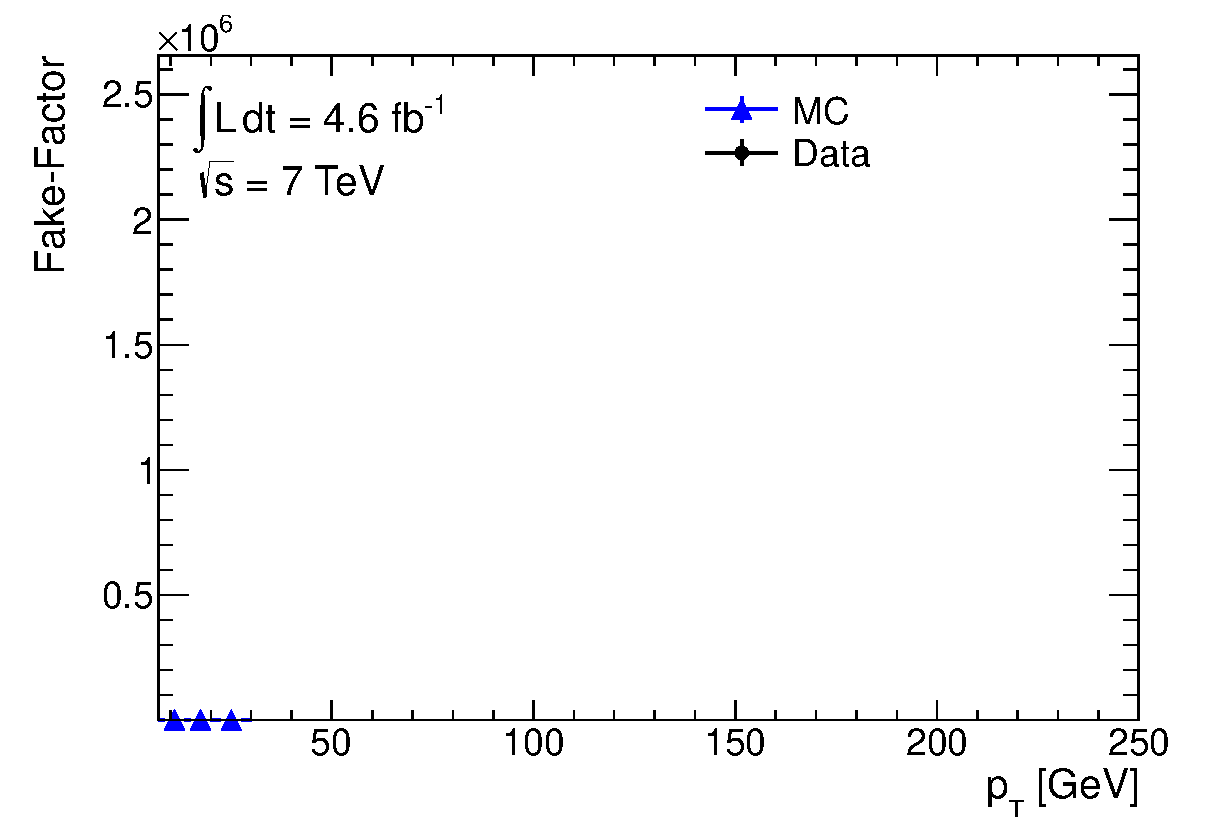
\includegraphics[width=0.47\textwidth]{FakeFactors/FF_ForwardMu_pt_B_lin}
%        }
%	\subfigure[Calorimeter-Tagged Muons]{
%            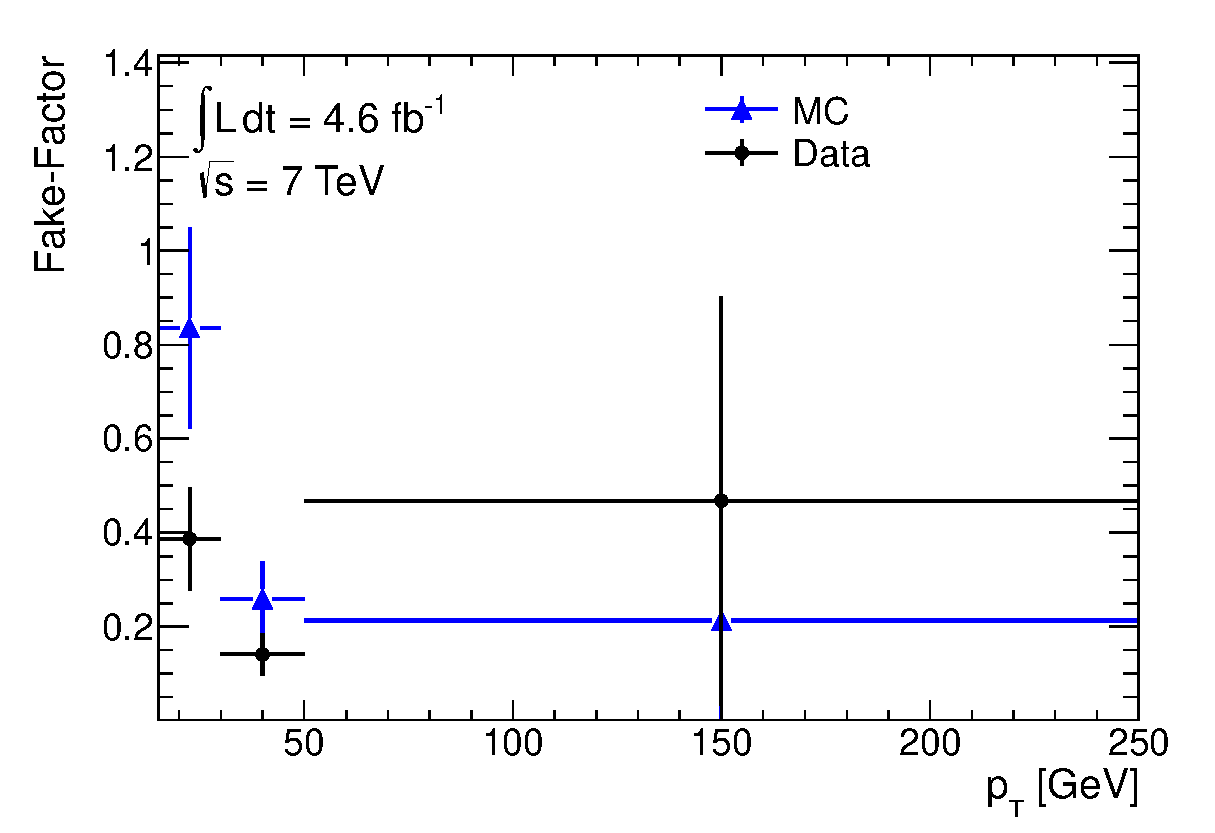
\includegraphics[width=0.47\textwidth]{FakeFactors/FF_CaloMu_pt_B_lin}
%        }
%	\subfigure[All Muons]{
%            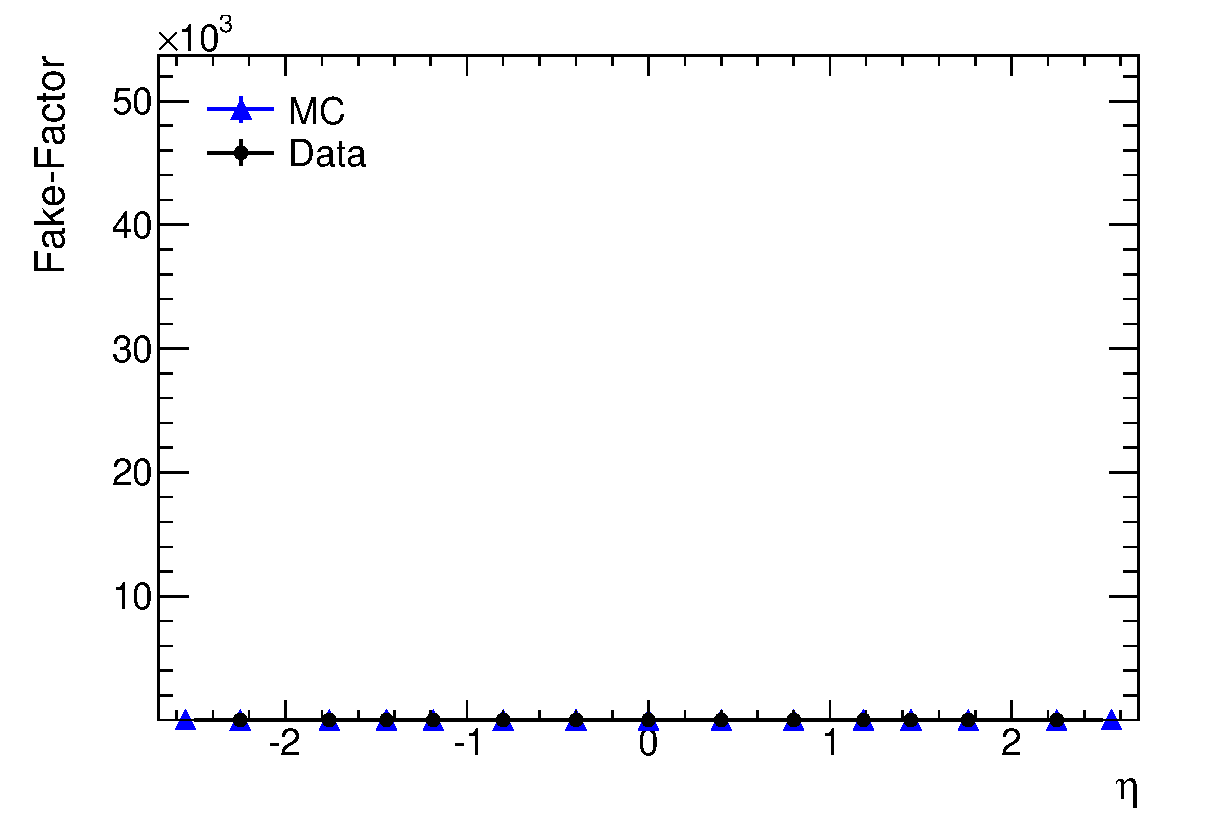
\includegraphics[width=0.47\textwidth]{FakeFactors/FF_AllMu_eta_B_lin}
%        }
%    \caption[Muon \FakeFactor s as a function of \pt\ and $\eta$ for 7~\tev\ data.]
%    {Muon \FakeFactor s as a function of \pt\ and $\eta$ for 7~\tev\ data. 
%    For the distributions as a function of \pt\, central, forward and calorimeter-tagged muons are shown
%    separately; for the $\eta$ distributions the \ffactor\ all electrons are
%    shown in the same plot.The black points show the \ffactor\ measured in
%    data; the blue triangles show the value estimated by \mc.}
%\label{fig:ff-mu-seven} 
%\end{figure}

\subsection{Statistical and Systematic Uncertainties}

The statistical error from the \ffactor\ measurement is propagated to the
background estimate by repeating the calculation with the \ffactor\ up and down
by the one-sigma statistical uncertainty. The variation of the predicted
background is then added in quadrature with the statistical uncertainty due to
limited numbers of observed $LLLJ$ and $LLJJ$ events. In cases where no $LLLJ$
or $LLJJ$ events are observed, the central value is taken as zero, and the
uncertainty is set to correspond to a 68\% confidence level upper limit on the
number of observed events of 1.29. This is scaled by the mean \ffactor\ for that
channel.

Systematic uncertainties are estimated by varying the criteria used to define
the \lljet s as follows:
\begin{itemize}
\item Increasing the inverted isolation requirement to $>$20\%, $>$30\%, and
$>$40\%. For the 7~\tev\ data, where both track and calroimeter isolation are
used, the requirements on the two isolations are varied
simultaneously.
\item Increasing the inverted \dzero-significance requirement to
$>4.0,>4.5,>5.0$.
%\item Requiring that the $J$ fail {\it either} the isolation {\it or} the
%identification (\dzero-significance) requirements, but not both.
\end{itemize}
The variations are designed to vary the composition of the different regions in
terms of the different sources of background leptons. Stability under these
variations indicates that the method is not sensitive to the composition of the
control region relative to the composition of the signal region. The final
background estimate is taken as the mean of the nominal background estimate and
the estimate obtained under each of these variations. The mean of the systematic
uncertainties is also taken; the systematic is taken as the RMS spread of the
estimates obtained from different variations.

In the \mmmm\ channel the number of observed $LLLJ$ and $LLJJ$ events is small,
and so the final background estimate is zero due to $N_LLJJ$ being larger than
$N_LLLJ$. In this case, the final result is taken as a truncated Gaussian, with
mean at zero and sigma equal to the estimated uncertainty. This procedure give a
conservative upper limit for the background.

\subsection{\mc\ Closure Test}

To demonstrate the validity of the background estimate method, a \mc\ closure
test is performed. The entire background estimate methodology described here is
applied to a \mc\ sample modelling \Zjets, \ttbar,
\singletop, \WZ\ and \WW\ backgrounds, to give a `background estimate' according
to the \mc. The \ffactor s are derived from the \mc, and are then applied
to $LLJJ$ and $LLLJ$ events from the \mc\ samples. The resulting `background
estimate' should then be in agreement with the number of $LLLL$ events passing the full
selection in the background \mc\ sample.


The results of the closure test are shown in~\tab{bg-est-mc-closure}. The
statistical uncertainties on the 8~\tev\ estimates are much larger, owing to the
size of the available \mc\ samples at 8~\tev\ being far smaller. In all cases, the
background estimate from \mc\ obtained using the \ffactor\ method is in good
agreement with the number of $LLLL$ events in the \mc.

\begin{table}
\small
\begin{tabular}{lcccc}
\hline\hline
    & \eeee & \mmmm & \eemm & \llll \\
\hline
\underline{\bf 7~\tev, \ZZ\ Selection} \\
$N_{BG}$ (\FFactor\ method) &  0.83 $\pm$ 0.29 &  0.04 $\pm$ 0.02 &  0.94 $\pm$ 0.36 &  1.81 $\pm$ 0.46 \\
$N_{LLLL}$ &  0.69 $\pm$ 0.25 &  0.01 $\pm$ 0.01 &  0.79 $\pm$ 0.28 &  1.49 $\pm$ 0.37 \\
\hline
\underline{\bf 7~\tev, \ZZs\ Selection} \\
$N_{BG}$ &  4.22 $\pm$ 0.81 &  -0.01 $\pm$ 0.07  &  4.54 $\pm$ 0.83 &  8.75 $\pm$ 1.17 \\
$N_{LLLL}$ &  3.80 $\pm$ 0.92 &  0.06 $\pm$ 0.05 &  4.41 $\pm$ 0.92 &  8.26 $\pm$ 1.30 \\
\hline
\underline{\bf 8~\tev, \ZZ\ Selection} \\
$N_{BG}$ &  2.40 $\pm$ 2.01 &  0.19 $\pm$ 0.05 &  2.16 $\pm$ 1.95  &  4.74 $\pm$ 2.80 \\
$N_{LLLL}$ &  2.99 $\pm$ 2.58 &  0.04 $\pm$ 0.04 &  0.62 $\pm$ 0.17 &  3.66 $\pm$ 2.58 \\
\hline\hline
\end{tabular}
\caption{Results of the \mc\ closure test for the data driven background
estimate. }
\end{table}



\subsection{Results}

The number of observed $LLLJ$ and $LLJJ$ events, these quantities multiplied by
the \fakefactor\ (squared in the latter case), the estimated correction due to
contamination from \ZZ\ events, and the resulting background estimate are shown
in~\tab{bg-est-nominal-seven} for the `nominal' $J$ definition for the 7~\tev\
data and in~\tab{bg-est-nominal-eight} for the 8~\tev\ data. The background
estimates under each of the variations described in the previous section are
shown in~\tabs{bg-est-syst-seven}{bg-est-syst-weight}. The results are observed to be stable under
the systematic variations. The final datat-driven background estimates are shown
in~\tab{bg-est-final}.

\begin{table}[htbp]
\footnotesize
\renewcommand\arraystretch{1.2}
\centering
\begin{tabular}{l|c|c|c|c}
\hline\hline
 & \eeee\ & \mmmm\ & \eemm\ & \llll\ \\
\hline
$N_{LLLJ}$ &  166.00 $\pm$ 12.88 &  9.00 $\pm$ 3.00 &  114.00 $\pm$ 10.68 &  289.00 $\pm$ 17.00 \\
($+$) $N_{LLLJ} \times FF$ &  17.71 $\pm$ 1.60 &  5.60 $\pm$ 2.30 &  17.52 $\pm$ 2.95 &  40.83 $\pm$ 4.07 \\
%$N_{LLLJ} \times FF$ Up &  18.12 $\pm$ 1.62 &  6.90 $\pm$ 2.99 &  19.94 $\pm$ 3.82 &  44.96 $\pm$ 5.12 \\
%$N_{LLLJ} \times FF$ Down &  17.30 $\pm$ 1.57 &  4.30 $\pm$ 1.64 &  15.09 $\pm$ 2.14 &  36.70 $\pm$ 3.12 \\
($-$) $N_{LLLJ}^{ZZ,MC}  \times FF^2$&  0.80 $\pm$ 0.02 &  1.90 $\pm$ 0.07 &  3.09 $\pm$ 0.12 &  5.79 $\pm$ 0.15 \\
$N_{LLJJ}$ &  661.00 $\pm$ 25.71 &  11.00 $\pm$ 3.32 &  443.00 $\pm$ 21.05 &  1115.00 $\pm$ 33.39 \\
($-$) $N_{LLJJ} \times FF^{2}$ &  7.05 $\pm$ 0.36 &  1.58 $\pm$ 0.54 &  5.77 $\pm$ 0.53 &  14.39 $\pm$ 0.84 \\
% $N_{LLJJ} \times FF$ Up &  7.38 $\pm$ 0.38 &  1.97 $\pm$ 0.68 &  6.43 $\pm$ 0.71 &  15.79 $\pm$ 1.05 \\
%$N_{LLJJ} \times FF$ Down &  6.72 $\pm$ 0.35 &  1.22 $\pm$ 0.42 &  5.15 $\pm$ 0.40 &  13.09 $\pm$ 0.68 \\
($+$) $N_{LLJJ}^{ZZ,MC}  \times FF^2$&  0.01 $\pm$ 0.00 &  0.02 $\pm$ 0.01 &  0.02 $\pm$ 0.00 &  0.05 $\pm$ 0.01 \\
\hline
$N_{BG}$ &  9.88 $\pm$ 1.64 $^{+0.86}_{-0.05}$ &  2.14 $\pm$ 2.37 $^{+2.79}_{-0.49}$ &  8.68 $\pm$ 3.00 $^{+4.83}_{-1.18}$ &  20.70 $\pm$ 4.16 $^{+8.48}_{-1.72}$ \\
%$N_{LLLL}$ &  62.00 $\pm$ 7.87 &  85.00 $\pm$ 9.22 &  158.00 $\pm$ 12.57 &  305.00 $\pm$ 17.46 \\
%$N_{LLLL}^{ZZ MC}$ &  57.92 $\pm$ 0.44 &  84.30 $\pm$ 0.54 &  136.30 $\pm$ 0.94 &  278.52 $\pm$ 1.17 \\
\hline\hline
\end{tabular}
\renewcommand\arraystretch{1.}
\caption{\small Details of the background estimate for 20~\ifb\ of 8~\tev\ data. The first row
shows the number of observed \NLLLJ\ events. The second row shows this quantity
scaled by the \ffactor\ (applied on an event by event basis), and the third row
the MC estimated number of \ZZ\ events identified as \LLJJ, scaled by the
\fakefactor. The fourth and
fifth rows
show the number of observed \NLLJJ\ events, and the number of \NLLJJ\ events
scaled by the \ffactor, and the sixth row the estimated number of \ZZ\ events
identified as \LLLJ, scaled by the \ffactor. The resulting background estimate
is shown in the last row, and is the sum of the rows indicated with `$(+)$',
minus the sum of the rows indicated with `$(-)$'. The first error is due to
statistical uncertainty on the number of observed \LLLJ\ and \LLJJ\ events,
while the
second error is due to statistical uncertainty on the \ffactor.}
\label{bg-est-nominal-eight}
\end{table}

\subsection{Cross Check with Same-Sign Events}

An additional cross check of the background estimate is performed by estimating
the background using a data sample composed of events passing the full event
selection, but with one opposite-signed
\dilep\ pair and one same-signed \dilep\ pair (termed OS-SS). The irreducible backgrounds due
to \Zjets, \ttbar, \WW\ and \WZ\ events will contribute to the OS-SS selection at
the same rate as to the signal selection with two oppositely-signed pairs
(SS-SS). There will be significant contamination to this control region from \ZZ\ events where
one lepton has its charged misidentified. This is estimated from \mc, and
subtracted from the observed OS-SS events to give the background events. 

The number of observed events passing the OS-SS selection, the
estimated \ZZ\ contamination and the resulting background estimate are shown
in~\tab{bg-est-ss}. The results are in good agreement with the background
estimate from the \ffactor\ method.

\begin{table}
\centering
\footnotesize
  \begin{tabular}{lcccc}
    \hline\hline
    & \eeee & \mmmm & \eemm & \llll \\
    \hline
    Observed OS-SS Events & 8 & 0 & 16 & 24 \\
    Expected \ZZ\ OS-SS & 2.65 \errSym{0.10} & 0.03 \errSym{0.01} & 3.19 \errSym{0.16} & 5.95 \errSym{0.19} \\
    \hline
    Bckg. Estimate (OS-SS)  & 5.35 \errSym{2.83} & $<$ 1.27 & 12.81
    \errSym{4.00} & 18.05 \errSym{2.83} \\
    Bckg. Estimate (\ffactor) & \ZZEightTeVDDBgEstEEEE &
    \ZZEightTeVDDBgEstMMMM & \ZZEightTeVDDBgEstEEMM & \ZZEightTeVDDBgEstLLLL \\
    \hline\hline
  \end{tabular}
      \caption[Background estimate cross check using same-sign events.]
      {Background estimate cross check using same-sign events.}
\label{table:bg-est-ss}
\end{table}

\section{Background Shape}

Due to the lack of statistics in the background \mc\ samples it is not possible
to obtain a background shape using the full event selection. In the 7~\tev\
data, there are also not enough statistics in the data control regions to obtain
a background shape. For the 7~\tev\ analysis, the background shape is therefore
taken from \mc\ with a loosened selection. For the background shape, events are
required to have an opposite-sign pair of leptons passing all of the selection
requirements. The second pair is not required to be same-signed, and the lepton
isolation and \dzero\ significance requirements are not applied.  Apart from
this, the full event selection, including mass cuts, is applied.  Applying this
selection, sufficient statistics are obtained from \mc\ to give reasonable
shapes in distributions of interest (e.g. \Z\ boson mass and \pt, four-lepton
mass, four-lepton \pt).

To account for the different efficiencies in the loosened selection criteria in
events with a ``loose'' electron pair and a ``loose'' muon pair, events of each
type are scaled by the ratio of the number of events which pass the nominal
selection to the number of events which pass the loosened selection.  
The ``loose'' electron pair efficiency was measured to be 0.051
while the ``loose'' muon pair efficiency  was measured to be 0.012.  This
scaling is used to account for any difference in shape between events with the
a ``loose'' electron pair and a ``loose'' muon pair.  The distributions thus
obtained are then normaised to the data-driven
background estimates shown in~\tab{bg-est-final}. 
%The statistical error on the full
%data-driven estimate was propagated to the per bin estimates and combined with
%the statistical error on the histogram while the systematic error per bin was
%solely propagated from the data-driven estimate.  

For the 8~\tev\ analysis, the background shape is taken from data, using $LLJJ$
events where the lepton-like jets are treated as fully selected leptons.  The
events are weighted by the fake factors for the lepton-like jets, and the
overall normalisation of the distribution is scaled to the data-drive background
estimate as shown in~\tab{bg-est-final}.  
%The statistical error on the full data-driven estimate was propagated to the
%per bin estimates and combined with the statistical error on the histogram
%while the systematic error per bin was solely propagated from the data-driven
%estimate.

